\documentclass[../DoAn.tex]{subfiles}
\begin{document}

\section{Thiết kế kiến trúc}
\subsection{Mô hình hệ thống}
\label{subsection:Mô hình hệ thống}
Như đã giới thiệu và giải thích ở Chương \ref{chapter:Methodology}, hệ thống server sẽ được triển khai trên kiến trúc SoC với khả năng truy cập từ xa, trên cơ sở này người viết mặc định client và server sẽ hoạt động ở hai mạng LAN khác nhau. Thông thường việc giao tiếp giữa hai mạng LAN sẽ phụ thuộc vào việc mở cổng mạng trên tường lửa router. Tuy nhiên, việc cấu hình này sẽ cần sự can thiệp của nhà cung cấp mạng và điều này sẽ tạo thành sự bất tiện trong trải nghiệm người dùng. Chính vì vậy, một giải pháp tối ưu và linh hoạt hơn đó chính là client và server sẽ kết nối với một server trung gian trước để khởi tạo và tạo thành Mesh Network. Sau khi kết nối vào Mesh Network, các thiết bị có thể tiến hành gửi và nhận dữ liệu như khi cùng một mạng LAN và không bị rào cản bởi tường lửa, Hình \ref{fig:Mô hình hệ thống} minh họa về mô hình hệ thống khi sử dụng dịch vụ Tailscale làm kết nối trung gian giữa client và server.

\begin{figure}[H]
    \centering
    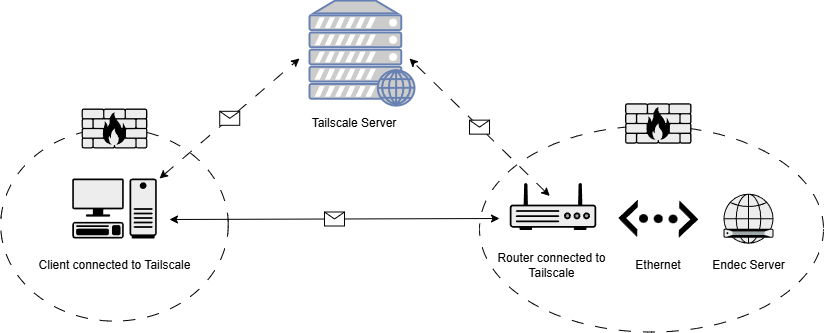
\includegraphics[width=0.8\textwidth, height=0.25\textheight, keepaspectratio]{Hinhve/Chuong 4/Device Diagram.png}
    \caption{Mô hình hệ thống}
    \label{fig:Mô hình hệ thống}
\end{figure}

Trên các thiết bị sử dụng hệ điều hành phổ biến thì có thể kết nối với server của Tailscale một cách trực tiếp, nhưng do Endec Server hướng tới việc tối ưu về mặt hiệu năng và độ trễ nên sẽ được thiết kế chạy trên baremetal. Việc chạy trên baremetal tuy cung cấp lợi thế rất lớn về hiệu năng và độ trễ nhưng cũng đồng thời gây ra trở ngại trong việc cấu hình kết nối với server Tailscale. Một giải pháp cho việc này đó chính là dùng một router làm cầu nối điều hướng luồng dữ liệu từ Endec Server đến server trung gian của Tailscale.

\subsection{Thiết kế tổng quan}

Việc sử dụng PL để tăng tốc khả năng mã hóa/giải mã và PS để điều khiển giao tiếp bên ngoài đòi hỏi sự chặt chẽ và tối ưu trong thiết kế giao tiếp giữa PS và PL bên cạnh việc tối ưu tác vụ xử lý tín hiệu trong nội bộ hai khối này. Hình \ref{fig:Endec Server data flow} minh họa cho luồng di chuyển của dữ liệu sau khi Endec Server nhận thành công dữ liệu từ client thông qua mạng lưới kết nối Internet đã được đề cập ở mục \ref{subsection:Mô hình hệ thống}.

\begin{figure}[H]
    \centering
    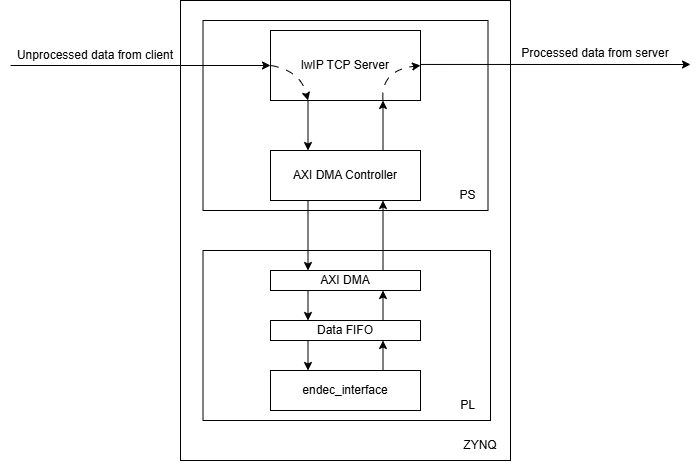
\includegraphics[width=0.9\textwidth, height=0.5\textheight, keepaspectratio]{Hinhve/Chuong 4/Endec Server data flow.png}
    \caption{Luồng dữ liệu trong Endec Server}
    \label{fig:Endec Server data flow}
\end{figure}

Các phần tiếp theo sẽ giải thích chi tiết về thiết kế và chức năng của từng khối chức năng trong đường đi của luồng dữ liệu.

\section{Thiết kế PL}

Thiết kế phần cứng cho bộ giải mã Viterbi đã trải qua nhiều thập kỷ phát triển, từ những kiến trúc đầu tiên dựa trên Radix-2 với các khối cơ bản như BMU (Branch Metric Unit), ACS (Add-Compare-Select) và bộ nhớ truy ngược (Traceback Memory) \cite{heller_viterbi_1971}\cite{feygin_survivor_1991}, đến các cải tiến hiệu suất bằng cách tăng bậc xử lý (radix). Trong môi trường FPGA, nơi tài nguyên phần cứng có thể được tùy chỉnh linh hoạt, việc chuyển từ Radix-2 sang Radix-4 trở thành xu hướng tối ưu nhờ khả năng xử lý 2 bit/chu kỳ, giảm độ trễ và tăng gấp đôi thông lượng so với Radix-2 truyền thống. Các nghiên cứu từ thập niên 90 \cite{black_140-mbs_1992} đã chứng minh Radix-4 phù hợp hơn với kiến trúc song song của FPGA, đồng thời tiết kiệm tài nguyên bộ nhớ và năng lượng nhờ giảm số chu kỳ tính toán.

Lợi thế lớn nhất của FPGA chính là khả năng xử lý đa luồng và thông lượng dữ liệu cao nhờ kiến trúc song song mềm dẻo. Trong nghiên cứu này, thiết kế PL tận dụng triệt để ưu thế trên thông qua kiến trúc giải mã Viterbi Radix-4, nơi mỗi chu kỳ xử lý đồng thời 2 bit dữ liệu. Để đảm bảo hiệu suất tổng thể, thiết kế còn tích hợp cơ chế pipeline tối ưu giữa các tầng xử lý và giao tiếp hiệu quả với PS thông qua AXI DMA cùng cơ chế điều phối luồng dữ liệu thông minh, tránh nghẽn cổ chai khi trao đổi dữ liệu tốc độ cao.

\begin{figure}[H]
    \centering
    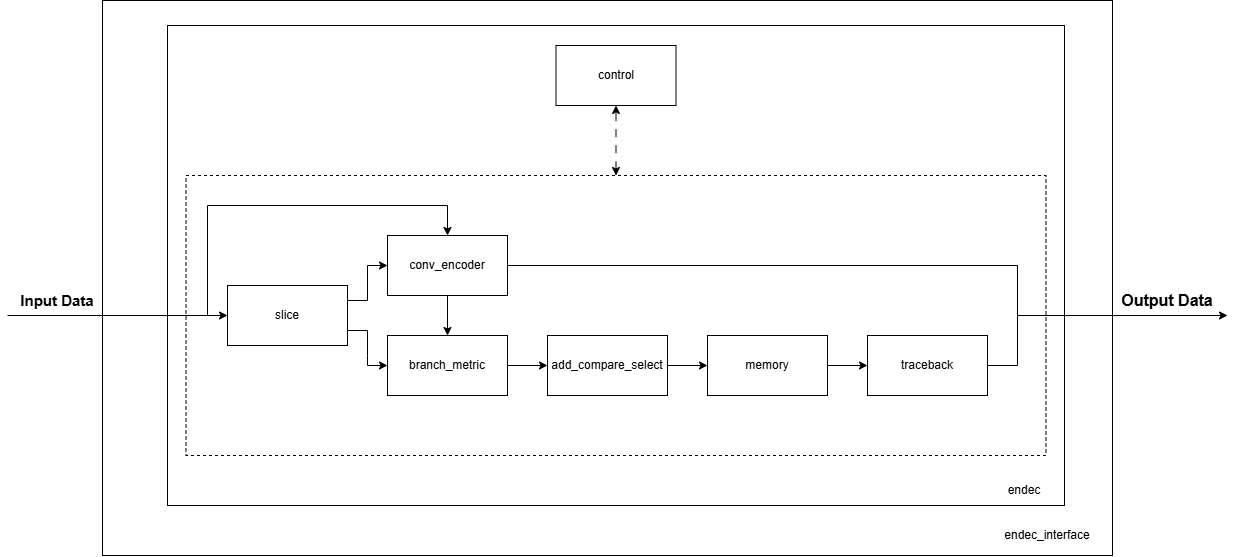
\includegraphics[width=0.9\textwidth, height=0.7\textheight, keepaspectratio]{Hinhve/Chuong 4/Endec data flow.png}
    \caption{Luồng dữ liệu trong khối endec\_interface}
    \label{fig:Luồng dữ liệu trong khối endec_interface}
\end{figure}

Hình \ref{fig:Luồng dữ liệu trong khối endec_interface} minh họa chi tiết luồng dữ liệu trong khối PL được thiết kế một cách có chủ đích và tỉ mỉ với đặc tính tuyến tính thể hiện rõ rệt. Đặc điểm thiết kế nổi bật này không chỉ mang lại hai lợi ích quan trọng hàng đầu mà còn đảm bảo hiệu suất ổn định: (i) thời gian xử lý trở nên hoàn toàn có thể dự đoán được (deterministic), từ đó loại bỏ hoàn toàn nguy cơ xảy ra hiện tượng treo hệ thống ngoài ý muốn trong điều kiện vận hành thực tế - đây chính là một yếu tố then chốt và không thể thiếu đối với các hệ thống thời gian thực yêu cầu độ tin cậy cao; (ii) kiến trúc pipeline được áp dụng nhất quán và xuyên suốt giữa các khối chức năng khác nhau, nhờ đó giúp tối đa hóa thông lượng xử lý của PL, đồng thời phát huy tối đa hiệu năng phần cứng sẵn có.


\subsection{Thiết kế khối endec\_interface}
\label{subsection:Thiết kế khối endec_interface}

\begin{figure}[H]
    \centering
    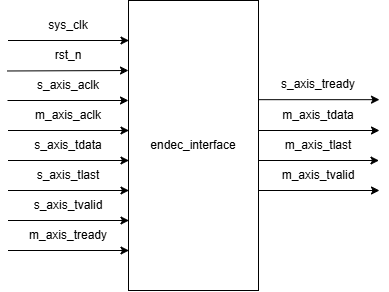
\includegraphics[width=0.75\textwidth, height=0.2\textheight, keepaspectratio]{Hinhve/Chuong 4/endec interface.png}
    \caption{Sơ đồ khối endec\_interface}
\end{figure}

\begin{table}[H]
\centering
    \caption{Tín hiệu vào/ra khối endec\_interface}
    \begin{tabular}{|p{0.28\linewidth}|p{0.08\linewidth}|p{0.08\linewidth}|p{0.05\linewidth}|p{0.35\linewidth}|}
        \hline
        \textbf{Tên tín hiệu} & \textbf{Số bit}  & \textbf{Mảng}     & \textbf{I/O}   & \textbf{Chức năng} \\ \hline\hline
        sys\_clk  & 1   & 1     & I     & tín hiệu đồng bộ theo sườn dương \\ \hline
        rst\_n    & 1   & 1     & I     & thiết lập lại trạng thái ban đầu\\ \hline
        s\_axis\_aclk  & 1   & 1     & I     & tín hiệu đồng bộ theo sườn dương, dùng cho s\_axis \\ \hline
        m\_axis\_aclk  & 1   & 1     & I     & tín hiệu đồng bộ theo sườn dương, dùng cho m\_axis \\ \hline
        s\_axis\_tdata  & 64   & 1     & I     & dữ liệu dùng cho s\_axis \\ \hline
        s\_axis\_tlast  & 1   & 1     & I     & báo hiệu nhịp dữ liệu cuối cùng của s\_axis \\ \hline
        s\_axis\_tvalid  & 1   & 1     & I     & báo hiệu dữ liệu hợp lệ cho s\_axis \\ \hline
        m\_axis\_tready  & 1   & 1     & I     & báo hiệu sẵn sàng nhận dữ liệu cho m\_axis \\ \hline
        s\_axis\_tready  & 1   & 1     & O     & báo hiệu sẵn sàng nhận dữ liệu cho s\_axis \\ \hline
        m\_axis\_tdata  & 64   & 1     & O     & dữ liệu dùng cho m\_axis \\ \hline
        m\_axis\_tlast  & 1   & 1     & O     & báo hiệu nhịp dữ liệu cuối cùng của m\_axis \\ \hline
        m\_axis\_tvalid  & 1   & 1     & O     & báo hiệu dữ liệu hợp lệ cho m\_axis \\ \hline
        \end{tabular}
\end{table}

Khối endec\_interface đóng vai trò quan trọng như một giao diện trung gian kết nối giữa khối AXI DMA và khối endec, có nhiệm vụ chính là tiếp nhận dữ liệu được truyền theo giao thức AXI từ AXI DMA, sau đó thực hiện chuyển đổi sang định dạng phù hợp để khối endec có thể xử lý một cách hiệu quả. 

Về mặt cấu trúc, khối này được chia thành ba module chức năng chính bao gồm RX, endec và TX, trong đó mỗi module đều được thiết kế thành các tiến trình hoạt động độc lập nhằm đáp ứng tính chất hoạt động tách biệt và chuyên biệt của từng thành phần. Cơ chế hoạt động chi tiết của các tiến trình này, đặc biệt khi khối endec\_interface bắt đầu thiết lập quá trình giao tiếp với AXI DMA, được mô tả và thể hiện một cách rõ ràng, cụ thể trong Hình \ref{fig:Sơ đồ tuần tự khối endec_interface}.

\begin{figure}[H]
    \centering
    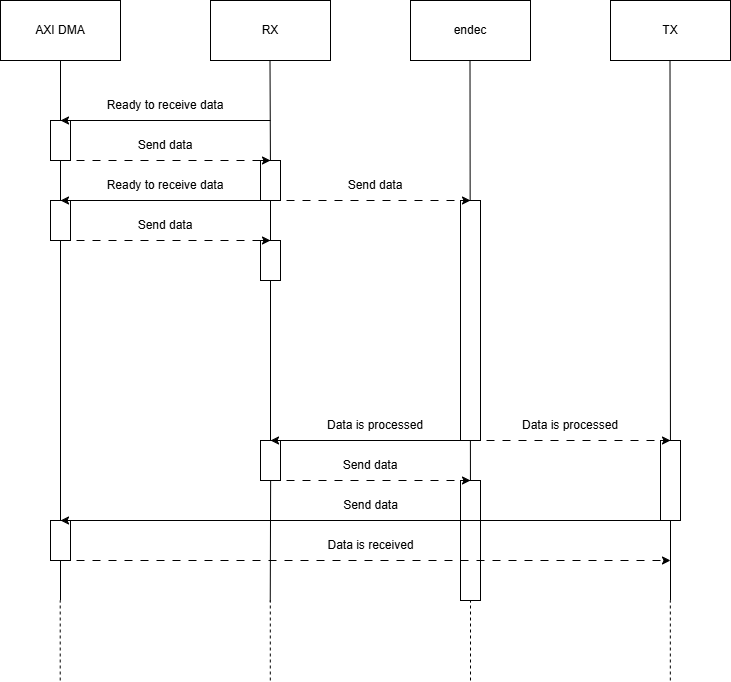
\includegraphics[width=0.85\textwidth, height=0.3\textheight, keepaspectratio]{Hinhve/Chuong 4/endec interface sequence.png}
    \caption{Sơ đồ tuần tự khối endec\_interface}
    \label{fig:Sơ đồ tuần tự khối endec_interface}
\end{figure}

Hình \ref{fig:Sơ đồ tuần tự khối endec_interface} minh họa rõ ưu điểm của kiến trúc đa luồng độc lập trong thiết kế: ngay khi khối endec bắt đầu xử lý dữ liệu hiện tại, khối RX đã có thể đồng thời tiếp nhận gói dữ liệu mới từ AXI DMA. Nhờ cơ chế hoạt động song song này, kể từ chu kỳ xử lý thứ hai trở đi, endec luôn có sẵn dữ liệu trong bộ đệm RX để xử lý ngay lập tức mà không phải chờ đợi thao tác truyền dữ liệu từ DMA, qua đó tối ưu hóa thông lượng hệ thống.

Để đảm bảo độ tin cậy, sau mỗi chu kỳ nhận dữ liệu từ RX và truyền dữ liệu đến TX, khối endec sẽ tự động thiết lập lại trạng thái ban đầu theo thiết kế. Cơ chế reset tuần hoàn này giúp hệ thống tránh được các lỗi tích lũy và duy trì tính ổn định trong quá trình vận hành liên tục.



\subsection{Thiết kế khối endec}

\begin{figure}[H]
    \centering
    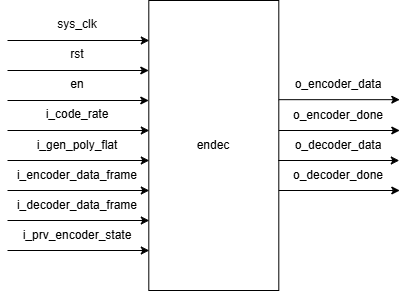
\includegraphics[width=0.75\textwidth, height=0.2\textheight, keepaspectratio]{Hinhve/Chuong 4/endec.png}
    \caption{Sơ đồ khối endec}
\end{figure}

\begin{table}[H]
\centering{}
    \caption{Tín hiệu vào/ra khối endec}
    \begin{tabular}{|p{0.28\linewidth}|p{0.08\linewidth}|p{0.08\linewidth}|p{0.05\linewidth}|p{0.35\linewidth}|}
        \hline
        \textbf{Tên tín hiệu} & \textbf{Số bit}  & \textbf{Mảng}     & \textbf{I/O}   & \textbf{Chức năng} \\ \hline\hline
        sys\_clk  & 1   & 1     & I     & tín hiệu đồng bộ theo sườn dương \\ \hline
        rst\_n    & 1   & 1     & I     & thiết lập lại trạng thái ban đầu\\ \hline
        en        & 1   & 1     & I     & tín hiệu cho phép hoạt động \\ \hline
        i\_code\_rate  & 1   & 1     & I     & cấu hình tốc độ mã \\ \hline
        i\_gen\_poly\_flat  & 27   & 1     & I     & cấu hình đa thức sinh \\ \hline
        i\_encoder\_data\_frame  & 192   & 1     & I     & khung dữ liệu cần mã hóa \\ \hline
        i\_decoder\_data\_frame  & 384   & 1     & I     & khung dữ liệu cần giải mã \\ \hline
        i\_prv\_encoder\_state  & 8   & 1     & I     & trạng thái cuối của thanh ghi dịch trong chu kỳ trước \\ \hline
        o\_encoder\_data  & 576   & 1     & O     & dữ liệu đã được mã hóa \\ \hline
        o\_encoder\_done  & 1   & 1     & O     & báo hiệu mã hóa hoàn thành \\ \hline
        o\_decoder\_data  & 128   & 1     & O     & dữ liệu đã được giải mã \\ \hline
        o\_decoder\_done  & 1   & 1     & O     & báo hiệu giải mã hoàn thành \\ \hline
        \end{tabular}
\end{table}

Khối endec đóng vai trò như là khối bao quát có vai trò liên kết tín hiệu giữa các khối con phía dưới và kết nối tín hiệu đầu vào đầu ra. Số lượng bit cho mỗi tín hiệu kết nối đã được người thiết kế tính toán sao cho tối ưu nhất với 64 bit dữ liệu trong giao thức truyền dữ liệu giữa endec\_interface và AXI DMA. Việc tổng số bit tín hiệu đầu vào/ra là bội số của 64 sẽ giúp toàn bộ chỗ chứa dữ liệu trong mỗi nhịp thời gian được tận dụng tối đa.

\subsection{Thiết kế khối control}

\begin{figure}[H]
    \centering
    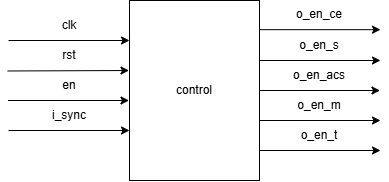
\includegraphics[width=0.75\textwidth, height=0.13\textheight, keepaspectratio]{Hinhve/Chuong 4/control.png}
    \caption{Sơ đồ khối control}
\end{figure}

\begin{table}[H]
\centering{}
    \caption{Tín hiệu vào/ra khối control}
    \begin{tabular}{|p{0.28\linewidth}|p{0.08\linewidth}|p{0.08\linewidth}|p{0.05\linewidth}|p{0.35\linewidth}|}
        \hline
        \textbf{Tên tín hiệu} & \textbf{Số bit}  & \textbf{Mảng}     & \textbf{I/O}   & \textbf{Chức năng} \\ \hline\hline
        clk  & 1   & 1     & I     & tín hiệu đồng bộ theo sườn dương \\ \hline
        rst   & 1   & 1     & I     & thiết lập lại trạng thái ban đầu\\ \hline
        en        & 1   & 1     & I     & tín hiệu cho phép hoạt động \\ \hline
        i\_sync  & 1   & 1     & I     & tín hiệu đồng bộ trạng thái \\ \hline
        o\_en\_ce  & 1   & 1     & O     & tín hiệu hoạt động cho khối conv\_encoder \\ \hline
        o\_en\_s  & 1   & 1     & O     & tín hiêu hoạt động cho khối slice \\ \hline
        o\_en\_acs  & 1   & 1     & O     & tín hiệu hoạt động cho khối add\_compare\_select \\ \hline
        o\_en\_m  & 1   & 1     & O     & tín hiệu hoạt động cho khối memory \\ \hline
        o\_en\_t  & 1   & 1     & O     & tín hiệu hoạt động cho khối traceback \\ \hline
        \end{tabular}
\end{table}

Khối control đóng vai trò trung tâm trong việc điều phối hoạt động của toàn hệ thống. Với đặc điểm phần lớn các khối chức năng đều sử dụng phần tử nhớ, việc điều khiển chính xác thời điểm kích hoạt/khoá các tín hiệu hoạt động là vô cùng quan trọng để đảm bảo quá trình nhận/gửi dữ liệu được đồng bộ hoá hoàn toàn. Để đạt được hiệu quả tối ưu, giải pháp triển khai thông qua FSM được lựa chọn. Hình \ref{fig:Trạng thái máy khối control} mô tả chi tiết các trạng thái hoạt động cũng như cơ chế chuyển đổi trạng thái của hệ thống, giúp đảm bảo tính ổn định và hiệu suất cao trong mọi tình huống vận hành.

\begin{figure}[H]
    \centering
    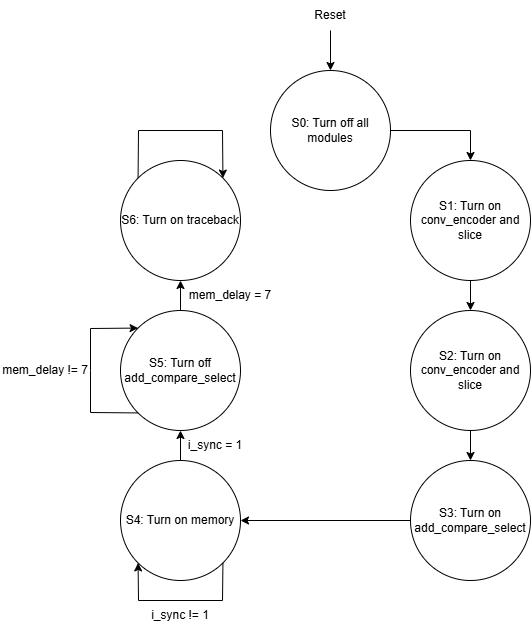
\includegraphics[width=0.8\textwidth, height=0.3\textheight, keepaspectratio]{Hinhve/Chuong 4/control state.png}
    \caption{Trạng thái máy khối control}
    \label{fig:Trạng thái máy khối control}
\end{figure}

Trong hệ thống PL, hoạt động chuyển mạch (switching activity) của các cổng logic giữa trạng thái 0 và 1 là nguồn tiêu thụ năng lượng chủ yếu. Do đó, cơ chế tắt động (clock gating/power gating) các khối chức năng khi không hoạt động không chỉ giảm đáng kể công suất tiêu thụ của PL mà còn nâng cao hiệu quả năng lượng cho toàn bộ hệ thống Endec Server. 

\subsection{Thiết kế khối slice}

\begin{figure}[H]
    \centering
    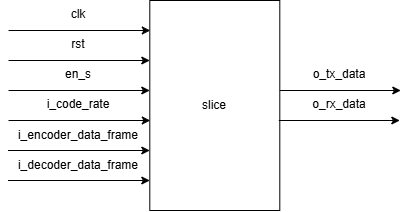
\includegraphics[width=0.75\textwidth, height=0.15\textheight, keepaspectratio]{Hinhve/Chuong 4/slice.png}
    \caption{Sơ đồ khối slice}
\end{figure}

\begin{table}[H]
\centering{}
    \caption{Tín hiệu vào/ra khối slice}
    \begin{tabular}{|p{0.28\linewidth}|p{0.08\linewidth}|p{0.08\linewidth}|p{0.05\linewidth}|p{0.35\linewidth}|}
        \hline
        \textbf{Tên tín hiệu} & \textbf{Số bit}  & \textbf{Mảng}     & \textbf{I/O}   & \textbf{Chức năng} \\ \hline\hline
        clk  & 1   & 1     & I     & tín hiệu đồng bộ theo sườn dương \\ \hline
        rst   & 1   & 1     & I     & thiết lập lại trạng thái ban đầu\\ \hline
        en\_s        & 1   & 1     & I     & tín hiệu cho phép hoạt động \\ \hline
        i\_code\_rate  & 1   & 1     & I     & báo hiệu thay đổi trạng thái \\ \hline
        i\_encoder\_data\_frame  & 192   & 1     & I     & khung dữ liệu cần mã hóa \\ \hline
        i\_decoder\_data\_frame  & 384   & 1     & I     & khung dữ liệu cần giải mã \\ \hline
        o\_tx\_data  & 1   & 1     & O     & nhóm bit cần mã hóa trong một bước thời gian \\ \hline
        o\_rx\_data  & 6   & 1     & O     & nhóm bit cần giải mã trong một bước thời gian \\ \hline
        \end{tabular}
\end{table}

Khối slice đảm nhận chức năng phân mảnh dữ liệu đầu vào, thực hiện chia tách các khung dữ liệu cần mã hóa/giải mã thành các nhóm bit con theo từng chu kỳ xử lý. Cơ chế phân chia này được thiết kế đặc biệt để đảm bảo sự tương thích tối ưu với các thuật toán xử lý tín hiệu ở các khối phía sau, đồng thời duy trì tính toàn vẹn của dòng dữ liệu trong suốt quá trình xử lý.

\subsection{Thiết kế khối conv\_encoder}

\begin{figure}[H]
    \centering
    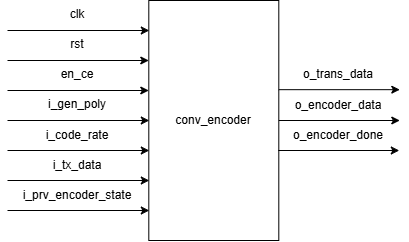
\includegraphics[width=0.75\textwidth, height=0.18\textheight, keepaspectratio]{Hinhve/Chuong 4/conv encoder.png}
    \caption{Sơ đồ khối conv\_encoder}
\end{figure}

\begin{table}[H]
\centering{}
    \caption{Tín hiệu vào/ra khối conv\_encoder}
    \begin{tabular}{|p{0.28\linewidth}|p{0.08\linewidth}|p{0.08\linewidth}|p{0.05\linewidth}|p{0.35\linewidth}|}
        \hline
        \textbf{Tên tín hiệu} & \textbf{Số bit}  & \textbf{Mảng}     & \textbf{I/O}   & \textbf{Chức năng} \\ \hline\hline
        clk  & 1   & 1     & I     & tín hiệu đồng bộ theo sườn dương \\ \hline
        rst   & 1   & 1     & I     & thiết lập lại trạng thái ban đầu\\ \hline
        en\_ce        & 1   & 1     & I     & tín hiệu cho phép hoạt động \\ \hline
        i\_gen\_poly  & 9   & 3     & I     & cấu hình đa thức sinh  \\ \hline
        i\_code\_rate  & 1   & 1     & I     & cấu hình tốc độ mã \\ \hline
        i\_tx\_data  & 1   & 1     & I     & dữ liệu cần mã hóa trong một bước thời gian\\ \hline
        i\_prv\_encoder\_state  & 8   & 1     & I     & trạng thái cuối của thanh ghi dịch trong chu kỳ trước \\ \hline
        o\_trans\_data  & 6   & 256x4     & O     & đầu ra tương ứng với một dịch chuyển \\ \hline
        o\_encoder\_data  & 576   & 1     & O     & dữ liệu đã được mã hóa \\ \hline
        o\_encoder\_done  & 1   & 1     & O     & báo hiệu mã hóa hoàn thành \\ \hline
        \end{tabular}
\end{table}

Khối conv\_encoder có nhiệm vụ chính là tìm đầu ra cho mỗi dịch chuyển giữa các trạng thái đối với cấu hình đa thức sinh tương ứng. Tuy nhiên, thuật toán tìm đầu ra này cũng chính là thuật toán mã hóa tích chập, chính vì vậy, ta có thể dễ dàng ứng dụng thêm một luồng mã hóa dữ liệu song song với luồng giải mã dữ liệu trong thiết kế. Việc xử lý song song này được mô hình hóa ở Hình \ref{fig:Luồng dữ liệu trong khối endec_interface} và Hình \ref{fig:Lưu đồ khối conv_encoder}. Giải thích chi tiết cho việc áp dụng này sẽ nằm ở mục \ref{section:Kết hợp mã hóa tích chập và giải mã Viterbi} trong Chương \ref{chapter:conclusion}.

\begin{figure}[H]
    \centering
    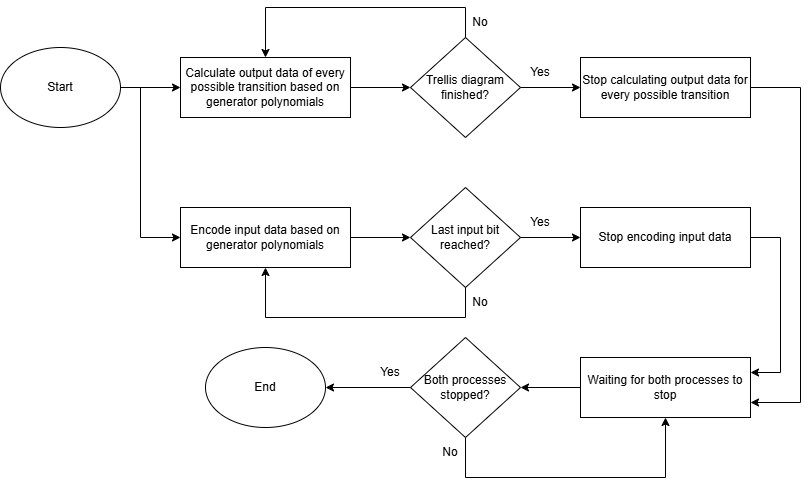
\includegraphics[width=0.9\textwidth, height=0.5\textheight, keepaspectratio]{Hinhve/Chuong 4/conv encoder flow chart.png}
    \caption{Lưu đồ khối conv\_encoder}
    \label{fig:Lưu đồ khối conv_encoder}
\end{figure}


\subsection{Thiết kế khối branch\_metric}
\begin{figure}[H]
    \centering
    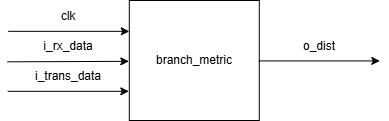
\includegraphics[width=0.75\textwidth, height=0.10\textheight, keepaspectratio]{Hinhve/Chuong 4/branch metric.png}
    \caption{Sơ đồ khối branch\_metric}
\end{figure}

\begin{table}[H]
\centering{}
    \caption{Tín hiệu vào/ra khối branch\_metric}
    \begin{tabular}{|p{0.28\linewidth}|p{0.08\linewidth}|p{0.08\linewidth}|p{0.05\linewidth}|p{0.35\linewidth}|}
        \hline
        \textbf{Tên tín hiệu} & \textbf{Số bit}  & \textbf{Mảng}     & \textbf{I/O}   & \textbf{Chức năng} \\ \hline\hline
        clk  & 1   & 1     & I     & tín hiệu đồng bộ theo sườn dương \\ \hline
        i\_rx\_data  & 6   & 1     & I     & đầu ra cần giải mã \\ \hline
        i\_trans\_data  & 6   & 256x4     & I     &  đầu ra của một dịch chuyển  \\ \hline
        o\_dist  & 3   & 256x4     & O     & khoảng cách Hamming của một dịch chuyển  \\ \hline
        \end{tabular}
\end{table}

Khối branch\_metric có nhiệm vụ so sánh đầu ra cần giải mã và đầu ra của dịch chuyển giữa các trạng thái để từ đó tính được khoảng cách Hamming.

\subsection{Thiết kế khối add\_compare\_select}

\begin{figure}[H]
    \centering
    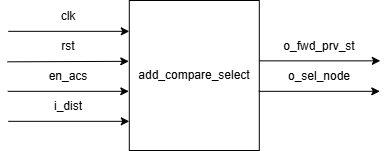
\includegraphics[width=0.75\textwidth, height=0.12\textheight, keepaspectratio]{Hinhve/Chuong 4/add compare select.png}
    \caption{Sơ đồ khối add\_compare\_select}
\end{figure}

\begin{table}[H]
\centering{}
    \caption{Tín hiệu vào/ra khối add\_compare\_select}
    \begin{tabular}{|p{0.28\linewidth}|p{0.08\linewidth}|p{0.08\linewidth}|p{0.05\linewidth}|p{0.35\linewidth}|}
        \hline
        \textbf{Tên tín hiệu} & \textbf{Số bit}  & \textbf{Mảng}     & \textbf{I/O}   & \textbf{Chức năng} \\ \hline\hline
        clk  & 1   & 1     & I     & tín hiệu đồng bộ theo sườn dương \\ \hline
        rst   & 1   & 1     & I     & thiết lập lại trạng thái ban đầu\\ \hline
        en\_acs  & 1   & 1     & I     & tín hiệu cho phép hoạt động \\ \hline
        i\_dist  & 3   & 256x4     & I     & khoảng cách Hamming của một dịch chuyển  \\ \hline
        o\_fwd\_prv\_st  & 8   & 256     & O     & nút được chọn trong bốn dịch chuyển khả thi đến một nút \\ \hline
        o\_sel\_node  & 8   & 1     & O     & nút có khoảng cách Hamming nhỏ nhất  \\ \hline
        \end{tabular}
\end{table}

Khối add\_compare\_select có nhiệm vụ tìm ra dịch chuyển và nút có khoảng cách Hamming nhỏ nhất để từ đó xây dựng nên sơ đồ lưới.

Đây là khối phức tạp nhất trong thiết kế PL, tuy có thuật toán khá đơn giản như minh họa ở Hình \ref{fig:Lưu đồ khối add_compare_select} nhưng với 1024 dịch chuyển và 256 nút cần xử lý và tính toán song song trong một bước thời gian thì việc tối ưu để triển khai thành công trên PL là một thách thức lớn. Vấn đề và cách giải quyết trong việc tối ưu và triển khai khối chức năng này sẽ được bàn chi tiết ở mục \ref{section:Tối ưu khối add_compare_select} trong Chương \ref{chapter:conclusion}.

\begin{figure}[H]
    \centering
    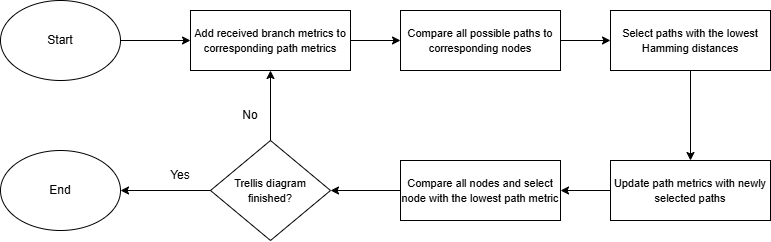
\includegraphics[width=0.9\textwidth, height=0.3\textheight, keepaspectratio]{Hinhve/Chuong 4/add compare select flow chart.png}
    \caption{Lưu đồ khối add\_compare\_select}
    \label{fig:Lưu đồ khối add_compare_select}
\end{figure}

\subsection{Thiết kế khối memory}

\begin{figure}[H]
    \centering
    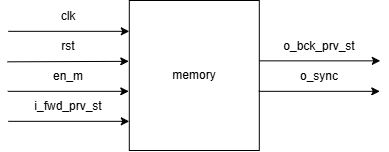
\includegraphics[width=0.75\textwidth, height=0.12\textheight, keepaspectratio]{Hinhve/Chuong 4/memory.png}
    \caption{Sơ đồ khối memory}
\end{figure}

\begin{table}[H]
\centering{}
    \caption{Tín hiệu vào/ra khối memory}
    \begin{tabular}{|p{0.28\linewidth}|p{0.08\linewidth}|p{0.08\linewidth}|p{0.05\linewidth}|p{0.35\linewidth}|}
        \hline
        \textbf{Tên tín hiệu} & \textbf{Số bit}  & \textbf{Mảng}     & \textbf{I/O}   & \textbf{Chức năng} \\ \hline\hline
        clk  & 1   & 1     & I     & tín hiệu đồng bộ theo sườn dương \\ \hline
        rst   & 1   & 1     & I     & thiết lập lại trạng thái ban đầu\\ \hline
        en\_m  & 1   & 1     & I     & tín hiệu cho phép hoạt động \\ \hline
        i\_fwd\_prv\_st  & 8   & 256     & I     & nút được chọn trong bốn dịch chuyển khả thi đến một nút chiều thuận  \\ \hline
        o\_bck\_prv\_st  & 8   & 256     & O     & nút được chọn trong bốn dịch chuyển khả thi đến một nút chiều nghịch \\ \hline
        o\_sync  & 1   & 1     & O     & tín hiệu đồng bộ trạng thái  \\ \hline
        \end{tabular}
\end{table}

Khối memory có nhiệm vụ lưu lại giá trị của các nút theo từng bước thời gian để xây dựng nên sơ đồ lưới. Sau khi lưu lại đủ số bước thời gian, khối memory sẽ gửi dữ liệu ở đầu ra để tiến hành truy ngược nhằm tìm đường đi có khoảng cách Hamming bé nhất cũng chính là đầu ra cần giải mã. Thuật toán này được minh họa chi tiết ở Hình \ref{fig:Lưu đồ khối memory}.

\begin{figure}[H]
    \centering
    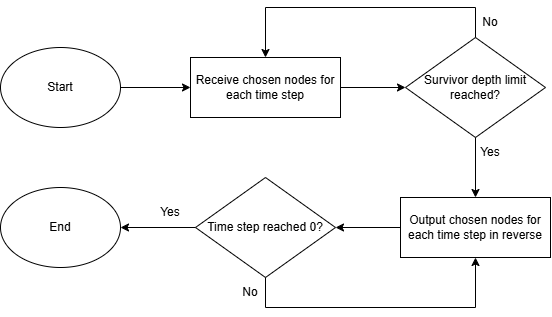
\includegraphics[width=0.75\textwidth, height=0.2\textheight, keepaspectratio]{Hinhve/Chuong 4/memory flow chart.png}
    \caption{Lưu đồ khối memory}
    \label{fig:Lưu đồ khối memory}
\end{figure}

Mặc dù thuật toán của khối này có nguyên lý hoạt động đơn giản, thách thức chính nằm ở bài toán thiết kế kiến trúc bộ nhớ. Với yêu cầu lưu trữ đồng thời dữ liệu của 256 nút cho mỗi bước thời gian và duy trì liên tục 64 bước thời gian, phương án triển khai thông thường sử dụng LUT và FF trên PL trở nên bất khả thi do giới hạn tài nguyên phần cứng \cite{noauthor_aup_nodate}. Giải pháp tối ưu hóa kiến trúc bộ nhớ nhằm cân bằng giữa hiệu năng xử lý và mức độ sử dụng tài nguyên sẽ được phân tích sâu tại mục \ref{section:Tối ưu khối memory} trong Chương \ref{chapter:conclusion}.

\subsection{Thiết kế khối traceback}

\begin{figure}[H]
    \centering
    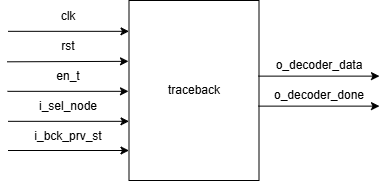
\includegraphics[width=0.75\textwidth, height=0.14\textheight, keepaspectratio]{Hinhve/Chuong 4/traceback.png}
    \caption{Sơ đồ khối traceback}
\end{figure}

\begin{table}[H]
\centering{}
    \caption{Tín hiệu vào/ra khối traceback}
    \begin{tabular}{|p{0.28\linewidth}|p{0.08\linewidth}|p{0.08\linewidth}|p{0.05\linewidth}|p{0.35\linewidth}|}
        \hline
        \textbf{Tên tín hiệu} & \textbf{Số bit}  & \textbf{Mảng}     & \textbf{I/O}   & \textbf{Chức năng} \\ \hline\hline
        clk  & 1   & 1     & I     & tín hiệu đồng bộ theo sườn dương \\ \hline
        rst   & 1   & 1     & I     & thiết lập lại trạng thái ban đầu\\ \hline
        en\_t  & 1   & 1     & I     & tín hiệu cho phép hoạt động \\ \hline
        i\_sel\_node  & 8   & 1     & I     & nút có khoảng cách Hamming nhỏ nhất  \\ \hline
        i\_bck\_prv\_st  & 8   & 256     & I     & nút được chọn trong bốn dịch chuyển khả thi đến một nút chiều nghịch \\ \hline
        o\_decoder\_data  & 128   & 1     & O     & dữ liệu đã được giải mã  \\ \hline
        o\_decoder\_done  & 1   & 1     & O     & báo hiệu giải mã hoàn thành  \\ \hline
        \end{tabular}
\end{table}

Từ dữ liệu của nút có khoảng cách Hamming nhỏ nhất từ khối add\_compare\_select và sơ đồ lưới lưu trữ dịch chuyển các nút từ khối memory, khối traceback sẽ truy ngược theo bước thời gian để tìm đầu vào cho dịch chuyển các nút để từ đó tìm được đầu ra cần giải mã.

\section{Thiết kế PS}

Khối PS có nhiệm vụ điều phối luồng dữ liệu giữa PL và client cần sử dụng dịch vụ mã hóa/giải mã dữ liệu. Luồng dữ liệu này được minh họa ở Hình \ref{fig:Luồng dữ liệu trong khối PS}.

\begin{figure}[H]
    \centering
    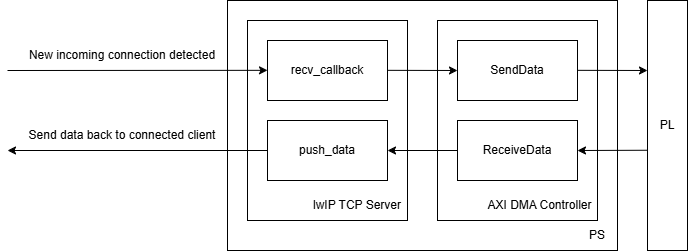
\includegraphics[width=0.9\textwidth, height=0.3\textheight, keepaspectratio]{Hinhve/Chuong 4/PS data flow.png}
    \caption{Luồng dữ liệu trong khối PS}
    \label{fig:Luồng dữ liệu trong khối PS}
\end{figure}

Dữ liệu thô nhận từ client trải qua quá trình tái định dạng để tuân thủ nghiêm ngặt chuẩn giao tiếp AXI trước khi truyền tới PL. Việc áp dụng chuẩn giao tiếp được tích hợp sẵn trong kiến trúc SoC mang lại ba lợi ích nổi bật: (i) tối ưu hóa thông lượng truyền dữ liệu và giảm thiểu độ trễ; (ii) đảm bảo tuyệt đối tính toàn vẹn dữ liệu thông qua cơ chế kiểm tra lỗi phần cứng; (iii) bảo vệ tín hiệu khỏi nhiễu điện từ nhờ các đường truyền được thiết kế tối ưu bởi nhà sản xuất - yếu tố then chốt trong các hệ thống giao tiếp tốc độ cao.  

\begin{table}[H]
\centering{}
    \caption{So sánh các phương thức truyền tải dữ liệu giữa PS và PL}
    \begin{tabular}{|p{0.17\linewidth} | p{0.18\linewidth}| p{0.24\linewidth}| p{0.27\linewidth}|}
        \hline
        \textbf{Phương thức} & \textbf{Thông lượng} & \textbf{Khối lượng dữ liệu}  & \textbf{Tài nguyên sử dụng}\\ \hline\hline
        AXI GPIO  & 10-100 MB/s  & Thấp, PS phải kết nối trực tiếp với từng chân tín hiệu   & Cao, PS phải điều khiển trực tiếp mọi khung truyền dữ liệu  \\ \hline
        AXI BRAM  & 300-600 MB/s & Thấp, bị giới hạn bởi cấu trúc của BRAM  & Cao, PS phải liên tục lấy mẫu và cập nhật dữ liệu cho BRAM   \\ \hline
        AXI DMA   & 1.2 GB/s & Cao, có thể lên tới 1024 bit trong một xung đồng hồ   & Thấp, PS chỉ phải khởi tạo và cấu hình DMA  \\ \hline
        \end{tabular}
    \label{table:So sánh các phương thức truyền tải dữ liệu giữa PS và PL}
\end{table}

Có rất nhiều cách để truyền dữ liệu giữa PS và PL như thể hiện ở Bảng \ref{table:So sánh các phương thức truyền tải dữ liệu giữa PS và PL} nhưng AXI DMA nổi bật lên nhờ sự tối ưu trong thông lượng và độ trễ khi truyền tải dữ liệu với khối lượng lớn. Bên cạnh đó, việc sử dụng AXI DMA còn giúp giải phóng tài nguyên PS khỏi việc di chuyển các khối dữ liệu để dành tài nguyên cho việc chạy lwIP TCP server. Đối với tài nguyên phần cứng tương đối hạn hẹp của PS trên PYNQ-Z2 \cite{noauthor_aup_nodate} thì việc ứng dụng AXI DMA cho giao tiếp giữa PS và PL trở thành điều bắt buộc. Hình \ref{fig:Lưu đồ khối PS} minh họa một cách trực quan thuật toán xử lý khi PS trong quá trình hoạt động.

\begin{figure}[H]
    \centering
    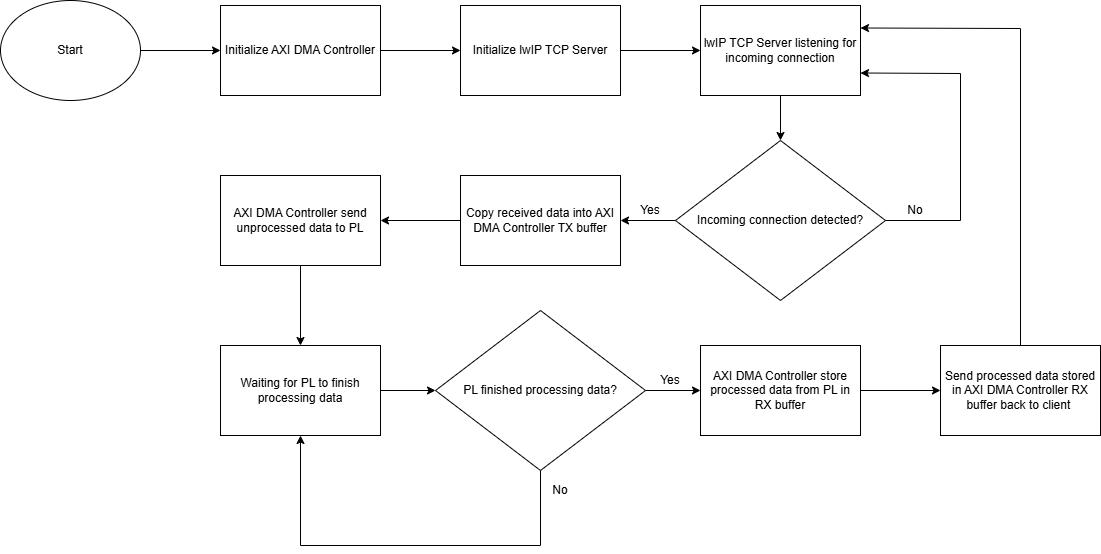
\includegraphics[width=0.9\textwidth, height=0.5\textheight, keepaspectratio]{Hinhve/Chuong 4/PS flow chart.png}
    \caption{Lưu đồ khối PS}
    \label{fig:Lưu đồ khối PS}
\end{figure}


\section{Triển khai và kiểm thử}

\subsection{Công cụ sử dụng}

\begin{table}[H]
\centering{}
    \caption{Danh sách phần mềm sử dụng}
    \begin{tabular}{|p{0.46\linewidth}|p{0.24\linewidth}|p{0.2\linewidth}|}
        \hline
        \textbf{Mục đích} & \textbf{Công cụ}  & \textbf{Ngôn ngữ} \\ \hline\hline
        Mô phỏng và kiểm thử  & Questa Sim   & SystemVerilog, Verilog           \\ \hline
        Tạo bộ dữ liệu chuẩn cho quá trình kiểm thử & MATLAB   & MATLAB          \\ \hline
        Tổng hợp và triển khai thiết kế trên phần cứng; Đọc dữ liệu từ ILA   & Vivado   & Tcl          \\ \hline
        Thiết kế và triển khai phần mềm nhúng  & Vitis Classic   & C          \\ \hline
        Đọc dữ liệu debug console qua USB  & PuTTY   &            \\ \hline
        Stress Test thông lượng TCP  & iPerf2   &            \\ \hline
        Chạy script truyền dữ liệu qua giao thức TCP và stress test thông lượng thực tế  & Powershell   & Python           \\ \hline
         Thiết lập Mesh Network  & Tailscale   &           \\ \hline
        \end{tabular}
\end{table}

\begin{table}[H]
\centering{}
    \caption{Danh sách phần cứng sử dụng}
    \begin{tabular}{|p{0.46\linewidth}|p{0.24\linewidth}|p{0.2\linewidth}|}
        \hline
        \textbf{Mục đích} & \textbf{Công cụ}  & \textbf{Nhà sản xuất} \\ \hline\hline
        Chạy Endec  Server  & PYNQ-Z2   & TUL           \\ \hline
        Router kết nối với Endec Server  & Beryl AX   & GL.iNet          \\ \hline
        Cung cấp kết nối mạng   & Modem E8372   & Huawei          \\ \hline
        Thử nghiệm thông lượng thuật toán MATLAB; Dùng làm client cho kết nối TCP   & Laptop Legion 5   & Lenovo          \\ \hline
        \end{tabular}
\end{table}

Với độ phức tạp của đề tài này, quá trình triển khai được chia thành ba giai đoạn chính: (i) thiết kế phần cứng trên PL, (ii) triển khai thiết kế PL lên phần cứng thực tế và (iii) lập trình nhúng cho PS. Nhằm đảm bảo độ tin cậy của hệ thống, sau khi hoàn thành mỗi giai đoạn, người viết sẽ tiến hành kiểm thử toàn diện các chức năng đã triển khai. Cách tiếp cận này giúp hạn chế tối đa các lỗi tiềm ẩn đồng thời cho phép phát hiện và xử lý sớm các vấn đề phát sinh trong quá trình phát triển hệ thống.

\subsection{Kiểm thử bằng mô phỏng}

Môi trường kiểm thử cho thiết kế cần kiểm tra (DUT) được dựa trên kiến trúc kiểm thử tổng quát (UVM) \cite{admin_uvm_nodate}. Tuy nhiên, vì nhiệm vụ chính của đề tài này là thiết kế và triển khai mà không phải kiểm thử nên môi trường kiểm thử đã được tối giản hóa và chỉ giữ lại những gì cần thiết nhất. Bên cạnh đó, việc kiểm thử cũng sẽ tập trung vào khả năng vận hành đúng theo thiết kế mà không đề cập tới khả năng chống lỗi của hệ thống nếu như bộ dữ liệu cố tình sai khác với thiết kế ban đầu.

\begin{figure}[H]
    \centering
    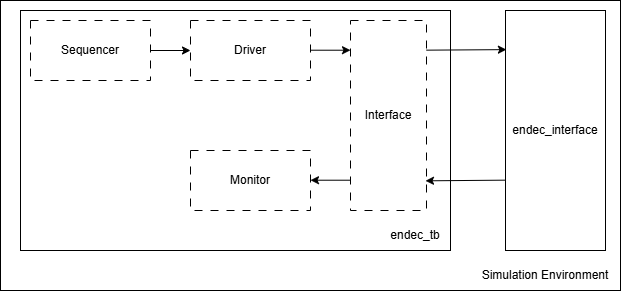
\includegraphics[width=0.75\textwidth, height=0.2\textheight, keepaspectratio]{Hinhve/Chuong 4/simulation block.png}
    \caption{Sơ đồ khối của môi trường kiểm thử bằng mô phỏng}
    \label{fig:Sơ đồ khối của môi trường kiểm thử}
\end{figure}

Hình \ref{fig:Sơ đồ khối của môi trường kiểm thử} mô tả kiến trúc tổng quan của môi trường kiểm thử. Cụ thể, hệ thống hoạt động theo cơ chế sau: Sequencer có nhiệm vụ chuyển đổi các dữ liệu mẫu (được tạo bằng MATLAB) sang định dạng tương thích với endec\_interface. Dữ liệu sau khi được xử lý sẽ được Driver truyền tới endec\_interface thông qua Interface. Song song đó, Monitor sẽ giám sát quá trình xử lý của endec\_interface và thu nhận kết quả phản hồi thông qua Interface. Quy trình kiểm thử được thực hiện bằng cách: (i) nạp dữ liệu đầu vào vào endec\_interface, (ii) so sánh kết quả đầu ra với bộ dữ liệu chuẩn. Phương pháp này cho phép đánh giá chính xác hiệu năng và độ tin cậy của endec\_interface.

Thiết kế này sau đó được triển khai trên phần mềm Questa Sim, kết quả của việc kiểm thử bằng mô phỏng được thể hiện ở Hình \ref{fig:Quá trình kiểm thử bằng mô phỏng}.

\begin{figure}[H]
    \centering
    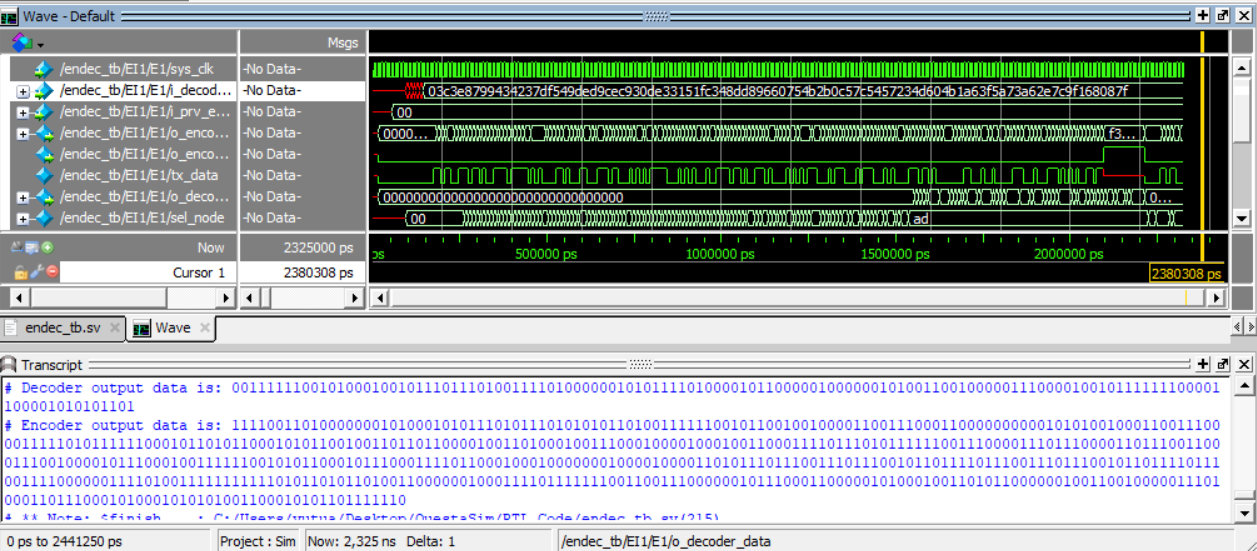
\includegraphics[width=\textwidth, height=0.33\textheight, keepaspectratio]{Hinhve/Chuong 4/simulation.png}
    \caption{Quá trình kiểm thử bằng mô phỏng}
    \label{fig:Quá trình kiểm thử bằng mô phỏng}
\end{figure}

Ví dụ minh họa cụ thể về quá trình kiểm thử bằng phương pháp mô phỏng được trình bày trong Hình \ref{fig:Quá trình kiểm thử bằng mô phỏng}. Trong thử nghiệm này, hệ thống đang được chạy với cấu hình thông số kỹ thuật bao gồm tốc độ mã hóa đặt ở mức 1/3, chiều dài ràng buộc được thiết lập là 9, đồng thời sử dụng bộ đa thức sinh tương ứng cho ba đầu ra ở dạng hệ 8 lần lượt là 557, 663 và 711. Kết quả mô phỏng thu được cho thấy tín hiệu đầu ra hoàn toàn khớp 100\% so với bộ dữ liệu mẫu tham chiếu được tạo ra từ MATLAB. Mặc dù đây mới chỉ là kết quả thử nghiệm trên một bộ dữ liệu cụ thể, nhưng với thiết kế đã được tổng quát hóa để có thể áp dụng cho nhiều trường hợp khác nhau, cùng với việc toàn bộ 704/704 bit dữ liệu đều khớp chính xác, kết quả này đã chứng minh một cách thuyết phục rằng thiết kế hiện tại hoạt động đúng như mong đợi và đạt được độ tin cậy cao.  


\subsection{Triển khai trên phần cứng và kiểm thử bằng ILA}
\subsubsection{Triển khai thiết kế PL}
\label{subsubsection:Triển khai thiết kế PL}
Sau khi kiểm thử mô phỏng về mặt chức năng thành công, thiết kế PL sẽ được nạp vào phần mềm Vivado để tiến hành tổng hợp thành các phần tử LUT và FF và triển khai các phần tử này trên phần cứng của PYNQ-Z2. Cũng tương tự như kiểm thử trên mô phỏng, việc kiểm thử trên phần cứng cũng bao gồm hai bước là: (i) nạp dữ liệu vào thiết kế cần kiểm thử và (ii) so sánh dữ liệu đầu ra với bộ dữ liệu mẫu.

Tuy nhiên, cấu trúc của thiết kế trên phần cứng sẽ khác với mô phỏng nên môi trường kiểm thử phần cứng cũng phải được thay đổi để phù hợp với sự khác biệt này. Hình \ref{fig:Sơ đồ khối môi trường kiểm thử phần cứng} mô tả môi trường kiểm thử thiết kế được triển khai trên phần cứng. Trong đó, khối giao tiếp ảo đầu vào/ra (Virtual Input/Output - VIO) có tác dụng gửi dữ liệu đầu vào tới endec\_interface (Hình \ref{fig:Thiết lập dữ liệu đầu vào trên VIO}) và dữ liệu đầu ra sẽ được ILA đọc và hiển thị dưới dạng tín hiệu sóng trong Vivado (Hình \ref{figure:Dữ liệu đọc được từ ILA}). 

\begin{figure}[H]
    \centering
    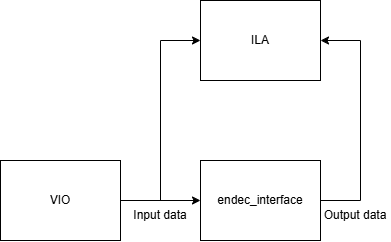
\includegraphics[width=0.75\textwidth, height=0.15\textheight, keepaspectratio]{Hinhve/Chuong 4/ILA block.png}
    \caption{Sơ đồ khối môi trường kiểm thử phần cứng}
    \label{fig:Sơ đồ khối môi trường kiểm thử phần cứng}
\end{figure}

\begin{figure}[H]
    \centering
    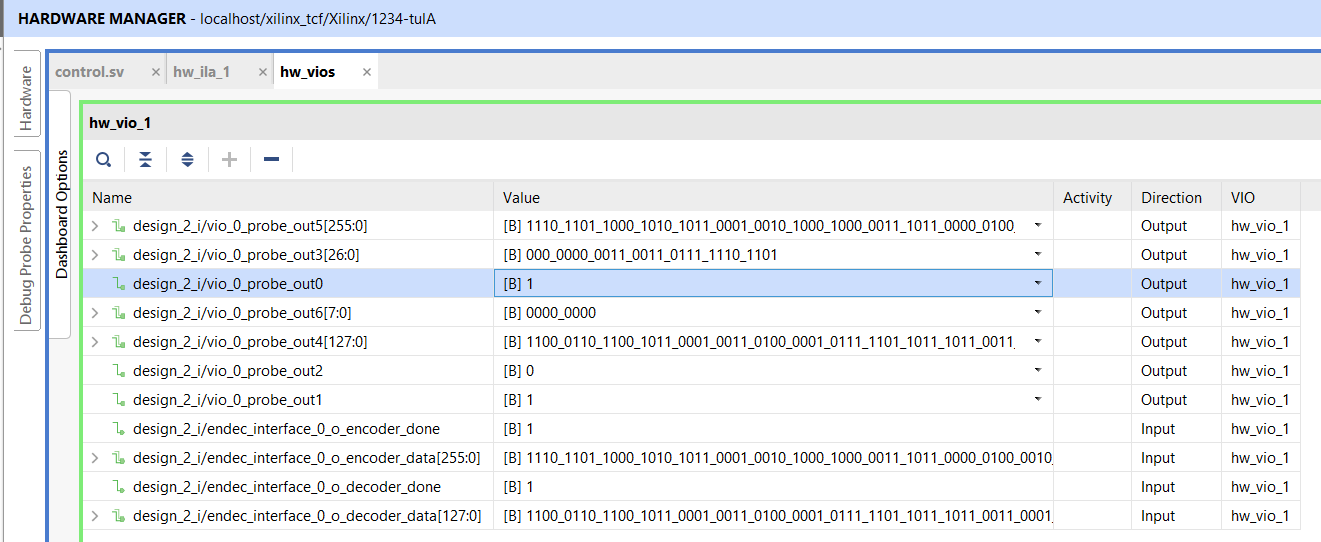
\includegraphics[width=0.95\textwidth, height=0.33\textheight, keepaspectratio]{Hinhve/Chuong 4/VIO.png}
    \caption{Thiết lập dữ liệu đầu vào trên VIO}
    \label{fig:Thiết lập dữ liệu đầu vào trên VIO}
\end{figure}

\begin{figure}[H]
    \centering
    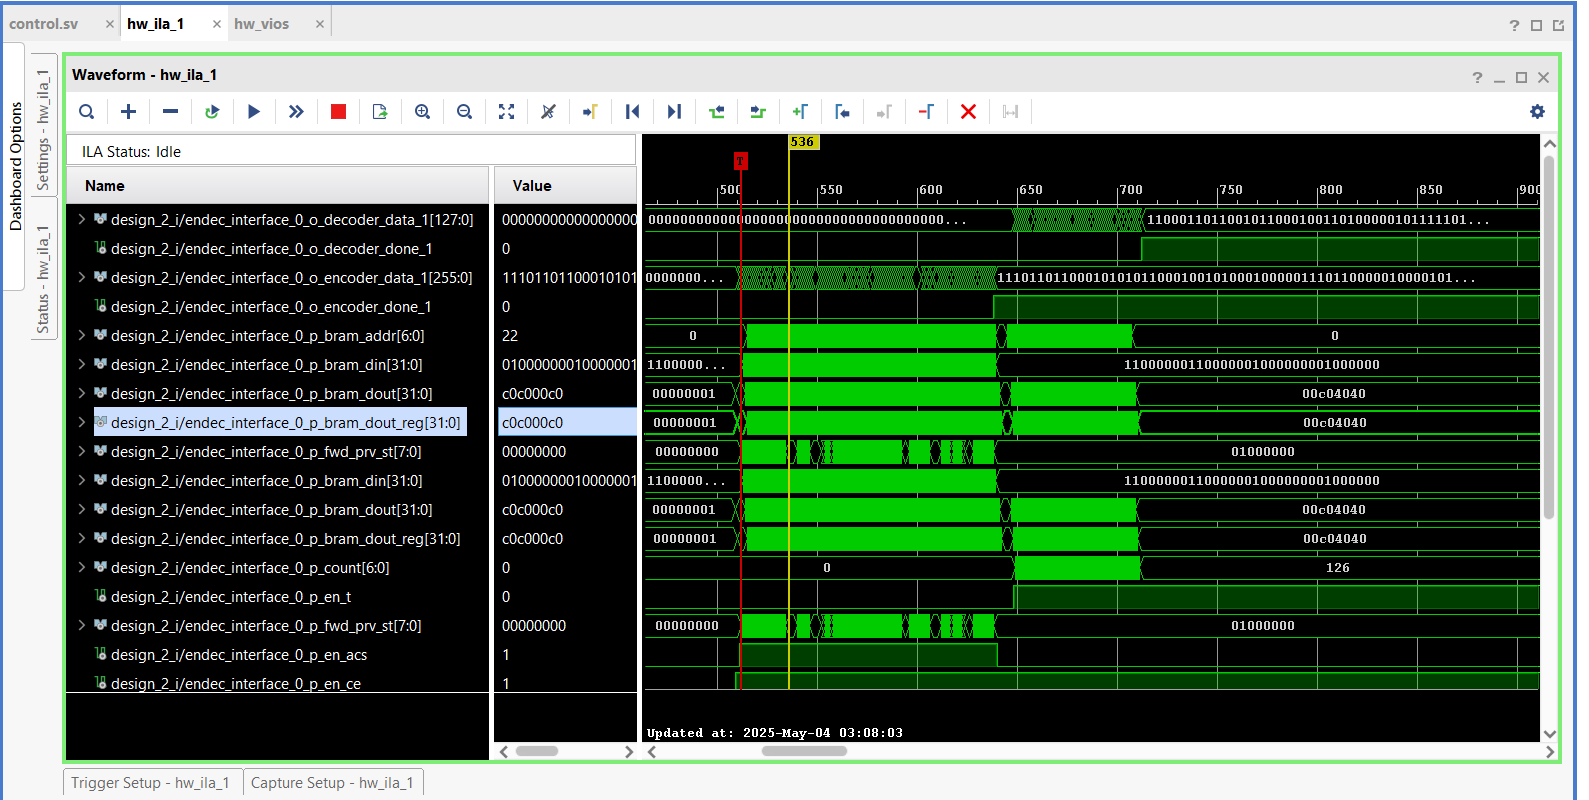
\includegraphics[width=0.95\textwidth, height=0.33\textheight, keepaspectratio]{Hinhve/Chuong 4/ILA raw data.png}
    \caption{Dữ liệu đọc được từ ILA}
    \label{figure:Dữ liệu đọc được từ ILA}
\end{figure}

Để sử dụng ILA như một Logic Analyzer đúng nghĩa, ta có thể tạo thêm đầu ra mới cho các khối chức năng và nối trực tiếp tín hiệu nội bộ trong các khối chức năng với đầu ra đó. Việc này tương đương với dùng que đo của Logic Analyzer để tiến hành đo đạc đường dây tín hiệu trong mạch thực tế. Các tín hiệu có tiền tố p\_ trong Hình \ref{figure:Dữ liệu đọc được từ ILA} đều đã được ILA đọc dữ liệu thông qua kỹ thuật này.

Thiết kế của PL trong mục này vẫn đang là dạng dữ liệu thô mà chưa được chuyển đổi cho tương thích với giao tiếp AXI. Tuy vậy nhưng các tín hiệu thu được bởi ILA trong Hình \ref{figure:Dữ liệu đọc được từ ILA} cũng hoàn toàn khớp với bộ dữ liệu mẫu từ MATLAB. Từ đó, ta có thể kết luận việc triển khai thiết kế PL trên phần cứng đã thành công và tiếp tục triển khai giai đoạn tiếp theo.

\subsubsection{Triển khai giao tiếp giữa PS và PL}

Phần này sẽ tiếp tục triển khai giao tiếp truyền dữ liệu giữa PS và PL trên cơ sở kiểm thử thành công trong việc sử dụng dữ liệu thô để truyền vào PL của phần \ref{subsubsection:Triển khai thiết kế PL}. Để việc truyền nhận dữ liệu giữa PL và PS diễn ra hiệu quả thì việc thiết kế giao thức kết nối là vô cùng quan trọng. Như đã trình bày ở mục \ref{subsection:Thiết kế khối endec_interface}, endec\_interface và khối AXI DMA sẽ giao tiếp thông qua giao thức AXI, quá trình kiểm thử chức năng của hệ thống cho đến bước hiện tại cũng đã diễn ra thành công. 

Ví dụ minh họa ở Hình \ref{fig:Phát hiện lỗi thông qua ILA} và Hình \ref{fig:Waveform sau khi sửa lỗi} sẽ chứng minh rõ nét nhất giá trị của việc ứng dụng ILA trong quá trình kiểm thử và sửa lỗi cho hệ thống.

\begin{figure}[H]
    \centering
    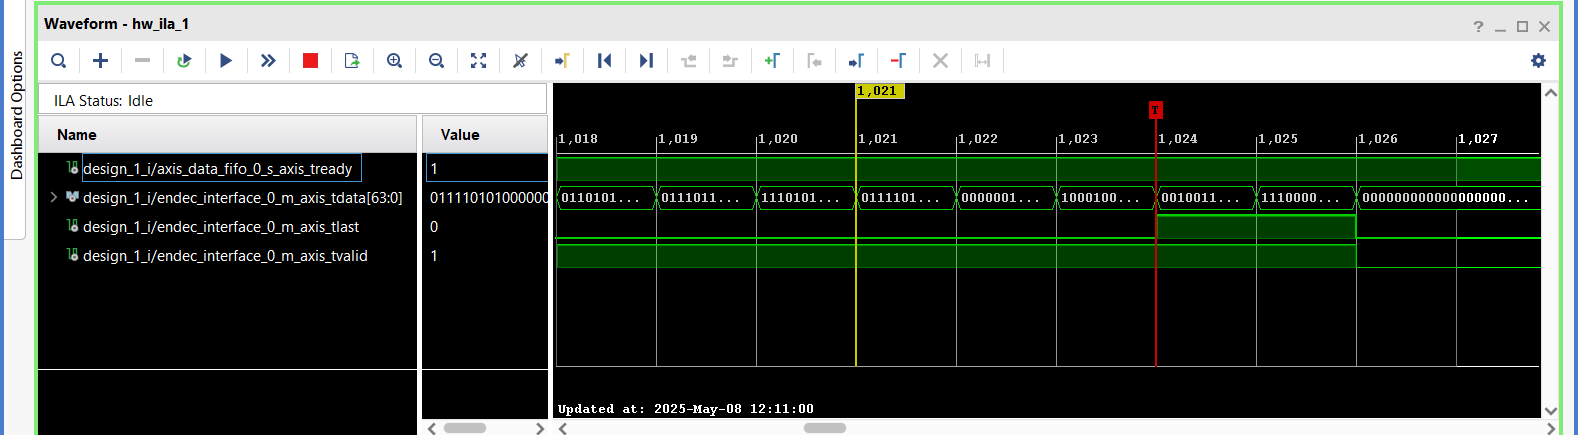
\includegraphics[width=\textwidth, height=0.33\textheight, keepaspectratio]{Hinhve/Chuong 4/ILA bug.png}
    \caption{Phát hiện lỗi thông qua ILA}
    \label{fig:Phát hiện lỗi thông qua ILA}
\end{figure}

Từ Hình \ref{fig:Phát hiện lỗi thông qua ILA} ta có thể thấy được lỗi trong chức năng TX của khối endec\_interface. Tín hiệu t\_last đã được bật lên ở hai thay vì một nhịp dữ liệu cuối. Điều này vi phạm giao thức AXI và lỗi này sẽ làm ảnh hưởng đến luồng dữ liệu giao tiếp từ PL đến PS và PS đến client.

\begin{figure}[H]
    \centering
    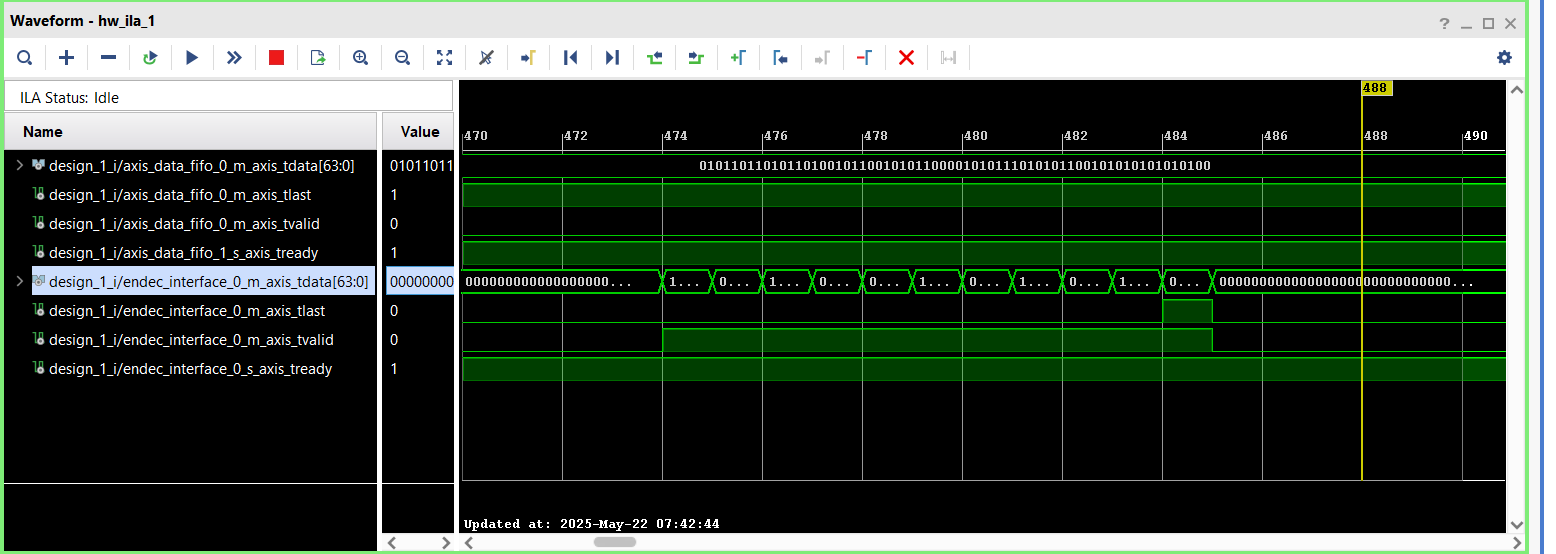
\includegraphics[width=\textwidth, height=0.33\textheight, keepaspectratio]{Hinhve/Chuong 4/ILA debug.png}
    \caption{Waveform sau khi sửa lỗi}
    \label{fig:Waveform sau khi sửa lỗi}
\end{figure}

Sau khi sửa lỗi, tín hiệu t\_last đã hoạt động đúng như mong đợi và có dạng như ở Hình \ref{fig:Waveform sau khi sửa lỗi}. Điều này cũng chỉ ra một điểm yếu rất lớn của việc kiểm thử bằng mô phỏng: môi trường mô phỏng mang tính chủ quan của người thiết kế và từ đó tính toàn diện của các trường hợp kiểm thử là không được đảm bảo. Chính vì vậy, việc sử dụng ILA trong quá trình phát triển và kiểm thử hệ thống là điều bắt buộc.

\subsection{Triển khai phần mềm nhúng và kiểm thử trực tiếp}
\label{subsection:Triển khai phần mềm nhúng và kiểm thử trực tiếp}

Hình \ref{fig:Luồng dữ liệu trong khối PS} và Hình \ref{fig:Lưu đồ khối PS} minh họa toàn bộ quy trình xử lý dữ liệu trong hệ thống. Sau khi hoàn thành các giai đoạn triển khai, kiểm thử và khắc phục lỗi trên PL, công đoạn cuối cùng là phát triển phần mềm nhúng cho PS. Phần mềm này có hai nhiệm vụ chính: (i) điều khiển khối AXI DMA thông qua AXI DMA Controller để quản lý luồng dữ liệu tốc độ cao giữa PS và PL, đồng thời (ii) thiết lập giao tiếp mạng với client thông qua lwIP TCP Server, tạo thành một hệ thống hoàn chỉnh có khả năng xử lý và truyền tải dữ liệu hiệu quả.

\begin{figure}[H]
    \centering
    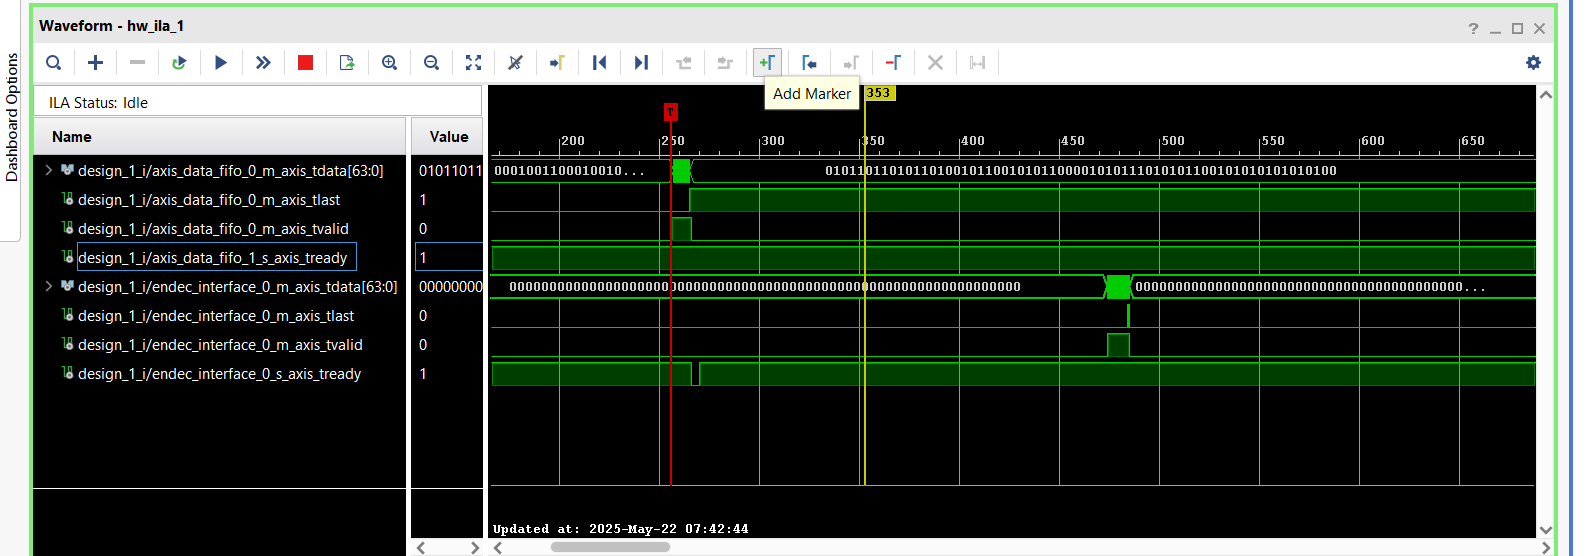
\includegraphics[width=\textwidth, height=0.33\textheight, keepaspectratio]{Hinhve/Chuong 4/ILA transfer.png}
    \caption{PS gửi một khung dữ liệu}
    \label{fig:PS gửi một khung dữ liệu}
\end{figure}

Hình \ref{fig:PS gửi một khung dữ liệu} minh họa chi tiết các tín hiệu giao tiếp được ghi lại bằng công cụ ILA trên bus dữ liệu kết nối giữa khối xử lý phần cứng PL và module AXI DMA. Quá trình này diễn ra sau khi bộ xử lý hệ thống PS hoàn tất việc cấu hình các thanh ghi của AXI DMA và thực hiện gửi thành công một khung dữ liệu đầy đủ từ bộ nhớ hệ thống sang phía PL. 

Từ kết quả phân tích tín hiệu ILA, có thể quan sát rõ ràng rằng phía PL đã nhận dữ liệu chính xác và đưa ra tín hiệu phản hồi sau khoảng thời gian xử lý tương đương với 209 chu kỳ xung nhịp. Khoảng thời gian đáp ứng này bao gồm cả độ trễ xử lý tín hiệu và thời gian truyền dẫn dữ liệu qua bus kết nối, cho thấy quá trình truyền nhận dữ liệu giữa hai khối đã diễn ra đúng như thiết kế.

\begin{figure}[H]
    \centering
    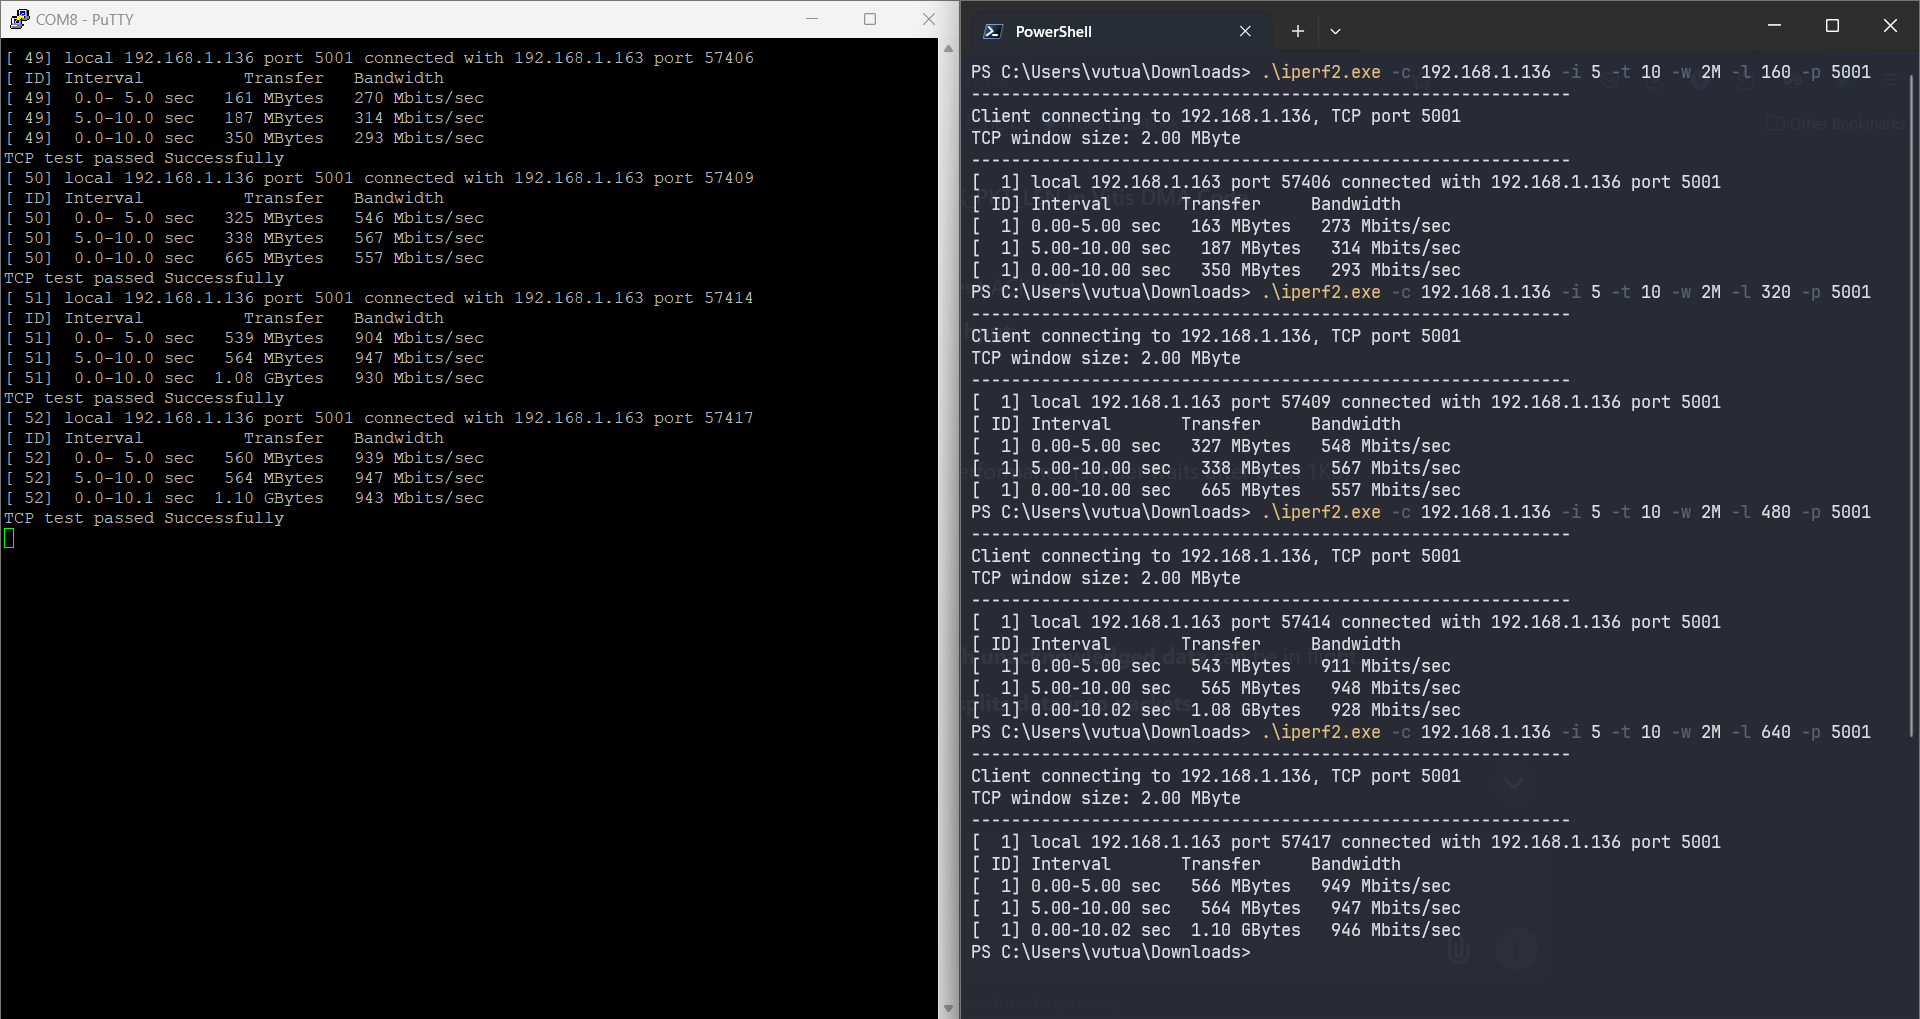
\includegraphics[width=\textwidth, height=0.4\textheight, keepaspectratio]{Hinhve/Chuong 4/tcp throughput.png}
    \caption{Tìm khung dữ liệu TCP cho thông lượng tối ưu}
    \label{fig:Tìm số dữ liệu tối ưu cho thông lượng}
\end{figure}

Mặc dù TCP được ưa chuộng nhờ khả năng đảm bảo tính toàn vẹn dữ liệu, giao thức này lại không tối ưu về mặt thông lượng do phải chịu chi phí xử lý (overhead) cho các cơ chế kiểm soát lỗi. Điều này dẫn đến yêu cầu quan trọng trong việc tối ưu hóa kích thước khung dữ liệu giữa client và Endec Server. Kết quả thử nghiệm hệ thống với kết nối Ethernet 1Gbps trong Hình \ref{fig:Tìm số dữ liệu tối ưu cho thông lượng} cho thấy: thông lượng đạt giá trị bão hòa 950 Mbps tại kích thước khung dữ liệu khoảng 500 byte. Để đạt được hiệu suất tối ưu, kích thước khung dữ liệu cần được chọn lớn hơn ngưỡng 500 byte này.

Sau khi tìm được cấu hình tối ưu cho kết nối giữa client và Endec Server, ta tiến hành thử nghiệm gửi tập tin dữ liệu từ client qua Endec Server. Hình \ref{fig:Client gửi một nhóm dữ liệu} cho thấy tín hiệu đã được PS tiếp nhận thành công từ client và truyền tới PL để xử lý. Tương tự như vậy, Hình \ref{fig:Kiểm thử kết nối với client} đã chứng tỏ được tín hiệu từ PL đã được PS tiếp nhận thành công và chuyển tiếp đến client. Kết quả cuối cùng mà client nhận được so sánh với bộ dữ liệu mẫu từ MATLAB và cho ra kết quả đúng 100\%.

\begin{figure}[H]
    \centering
    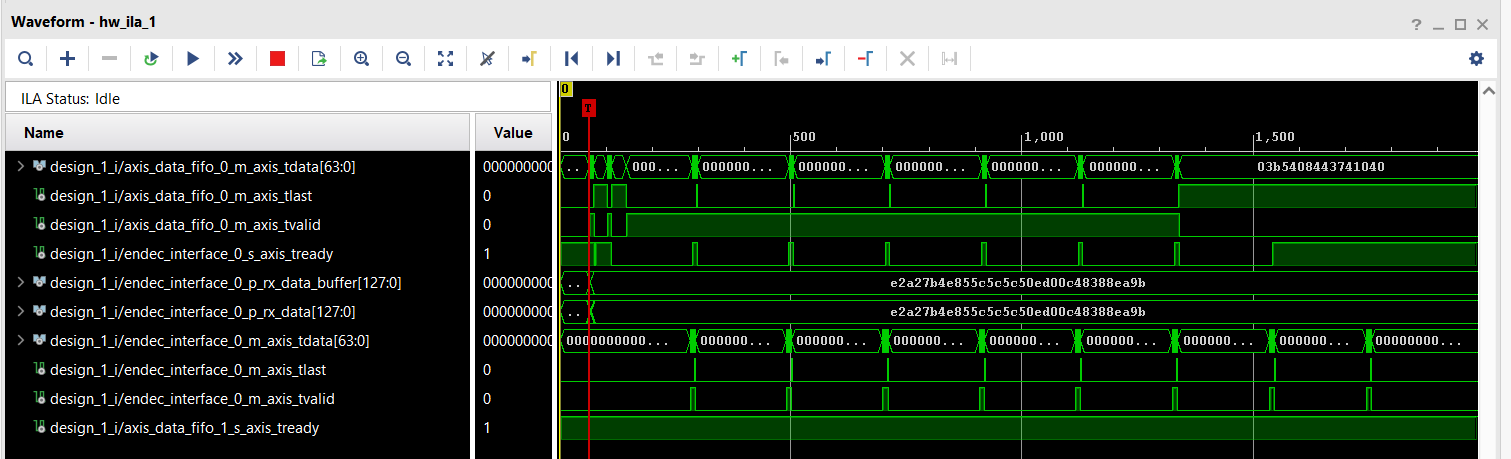
\includegraphics[width=\textwidth, height=0.33\textheight, keepaspectratio]{Hinhve/Chuong 4/ILA transaction.png}
    \caption{Client gửi một nhóm dữ liệu}
    \label{fig:Client gửi một nhóm dữ liệu}
\end{figure}

\begin{figure}[H]
    \centering
    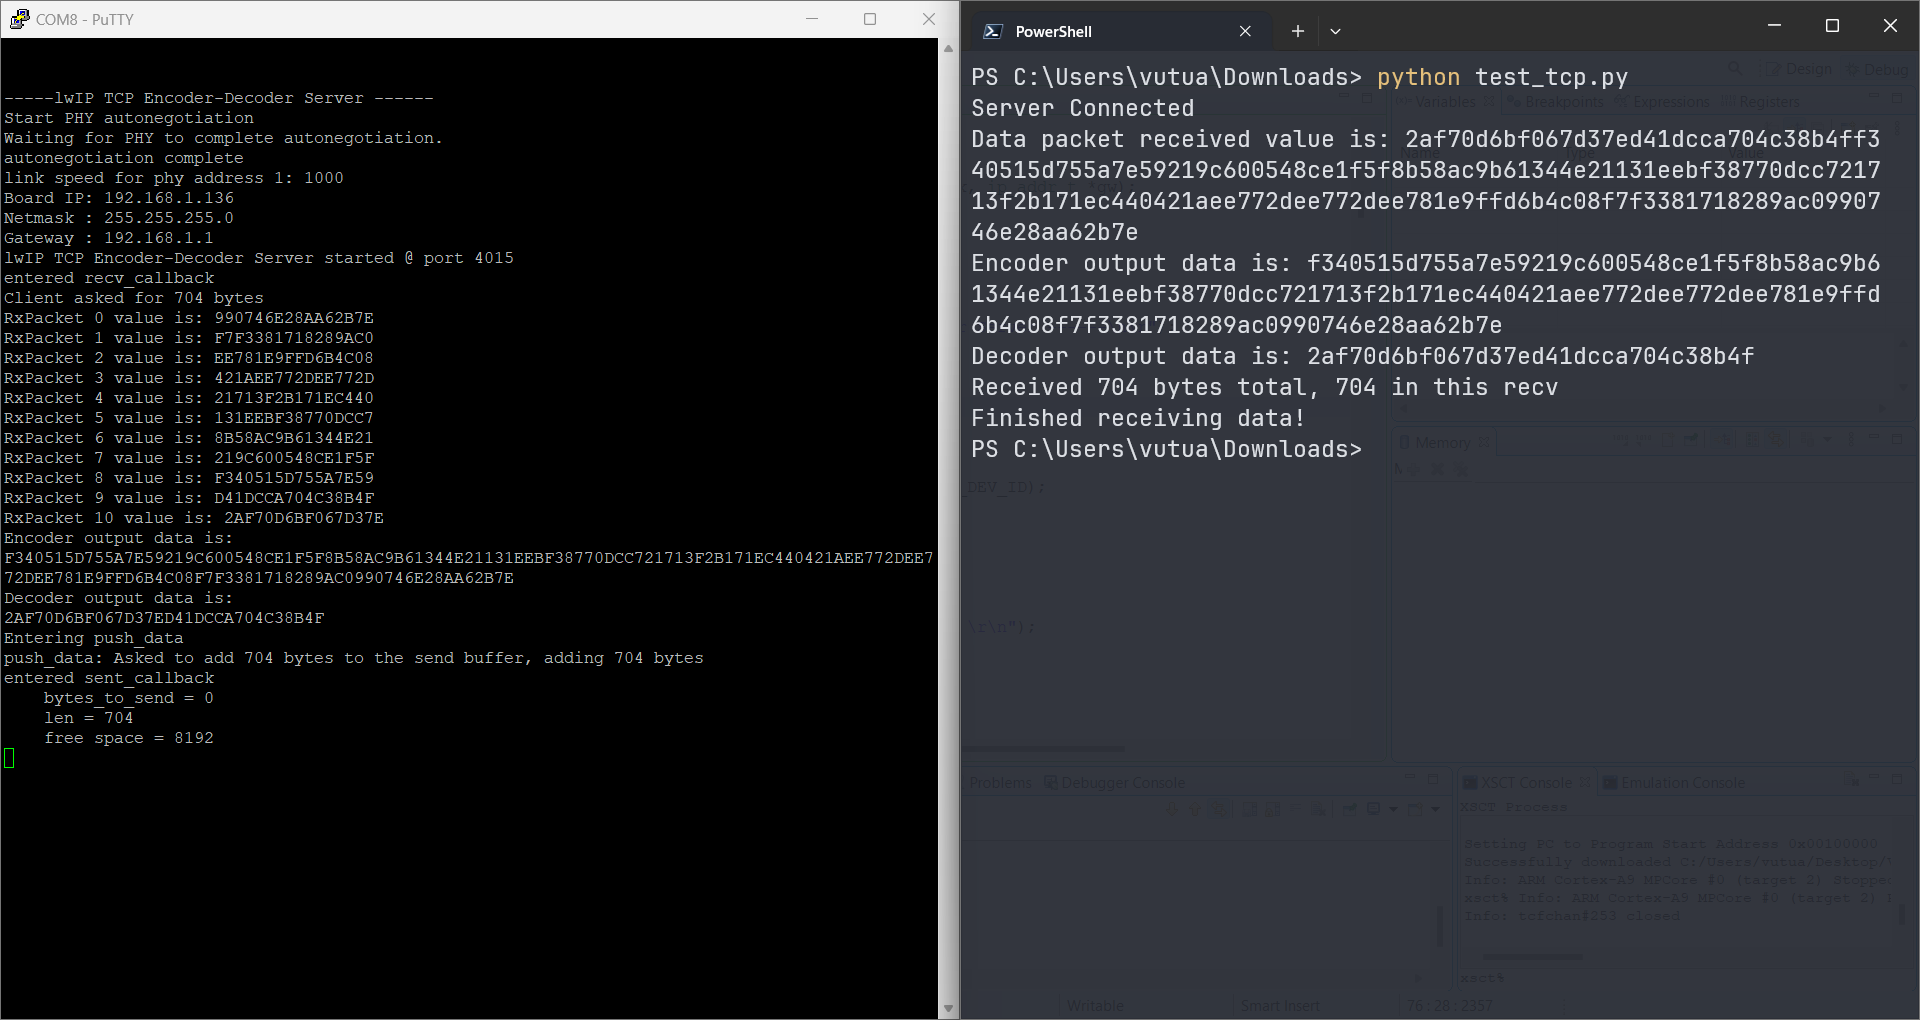
\includegraphics[width=\textwidth, height=0.4\textheight, keepaspectratio]{Hinhve/Chuong 4/packet test.png}
    \caption{Kiểm thử kết nối với client}
    \label{fig:Kiểm thử kết nối với client}
\end{figure}

Tiếp theo, ta tiến hành kiểm thử kết nối Tailscale. Endec Server được kết nối trực tiếp với router Beryl AX qua cổng Ethernet. Trong Hình \ref{fig:Kiểm thử client cùng mạng LAN}, client kết nối vào mạng GL-MT3000-159-5G (mạng Wi-Fi do router Beryl AX phát ra) và giao tiếp thành công với Endec Server – đây là trường hợp kết nối chung mạng LAN. Ở trường hợp thứ hai (Hình \ref{fig:Kiểm thử client kết nối với Tailscale}), dù client thuộc một mạng LAN khác, nhưng nhờ cả router Beryl AX và client cùng tham gia vào Mesh Network của Tailscale, việc truyền nhận dữ liệu giữa client và Endec Server vẫn diễn ra bình thường mà không cần mở cổng mạng trên router.

\begin{figure}[H]
    \centering
    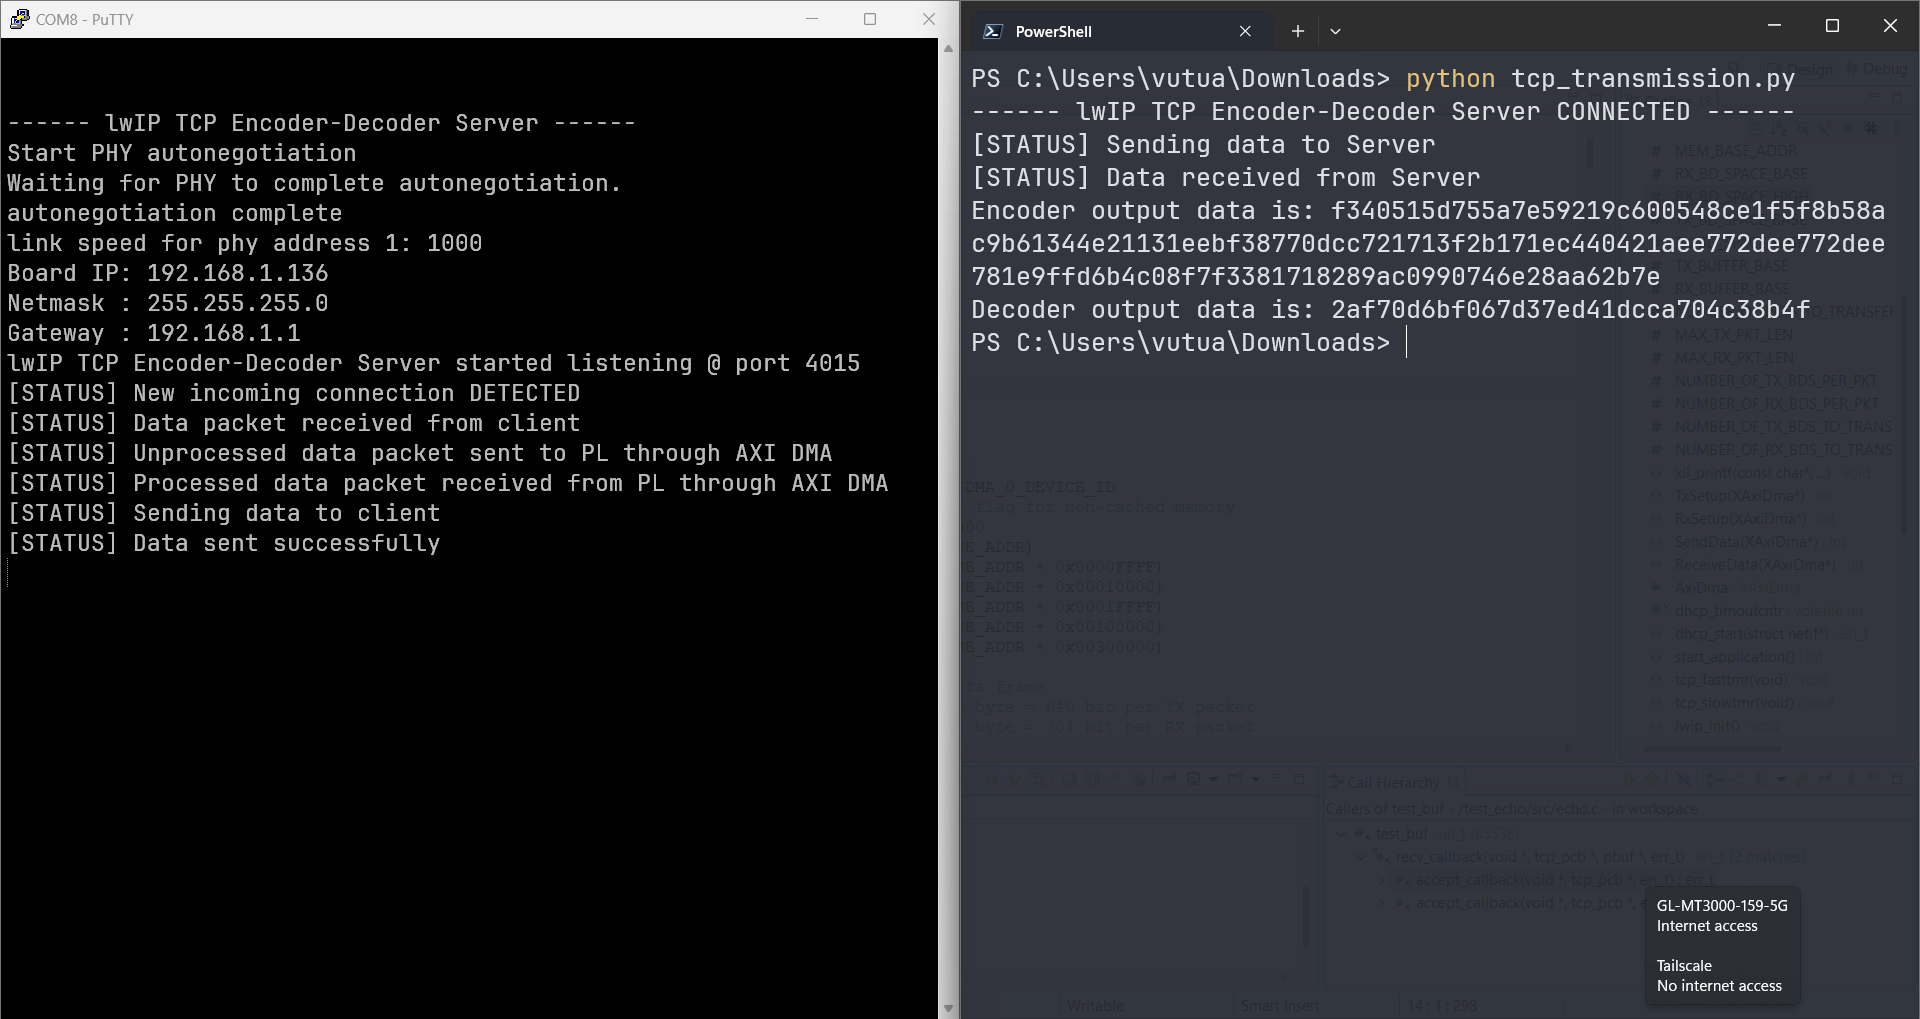
\includegraphics[width=\textwidth, height=0.4\textheight, keepaspectratio]{Hinhve/Chuong 4/lan.png}
    \caption{Kiểm thử client cùng mạng LAN}
    \label{fig:Kiểm thử client cùng mạng LAN}
\end{figure}

\begin{figure}[H]
    \centering
    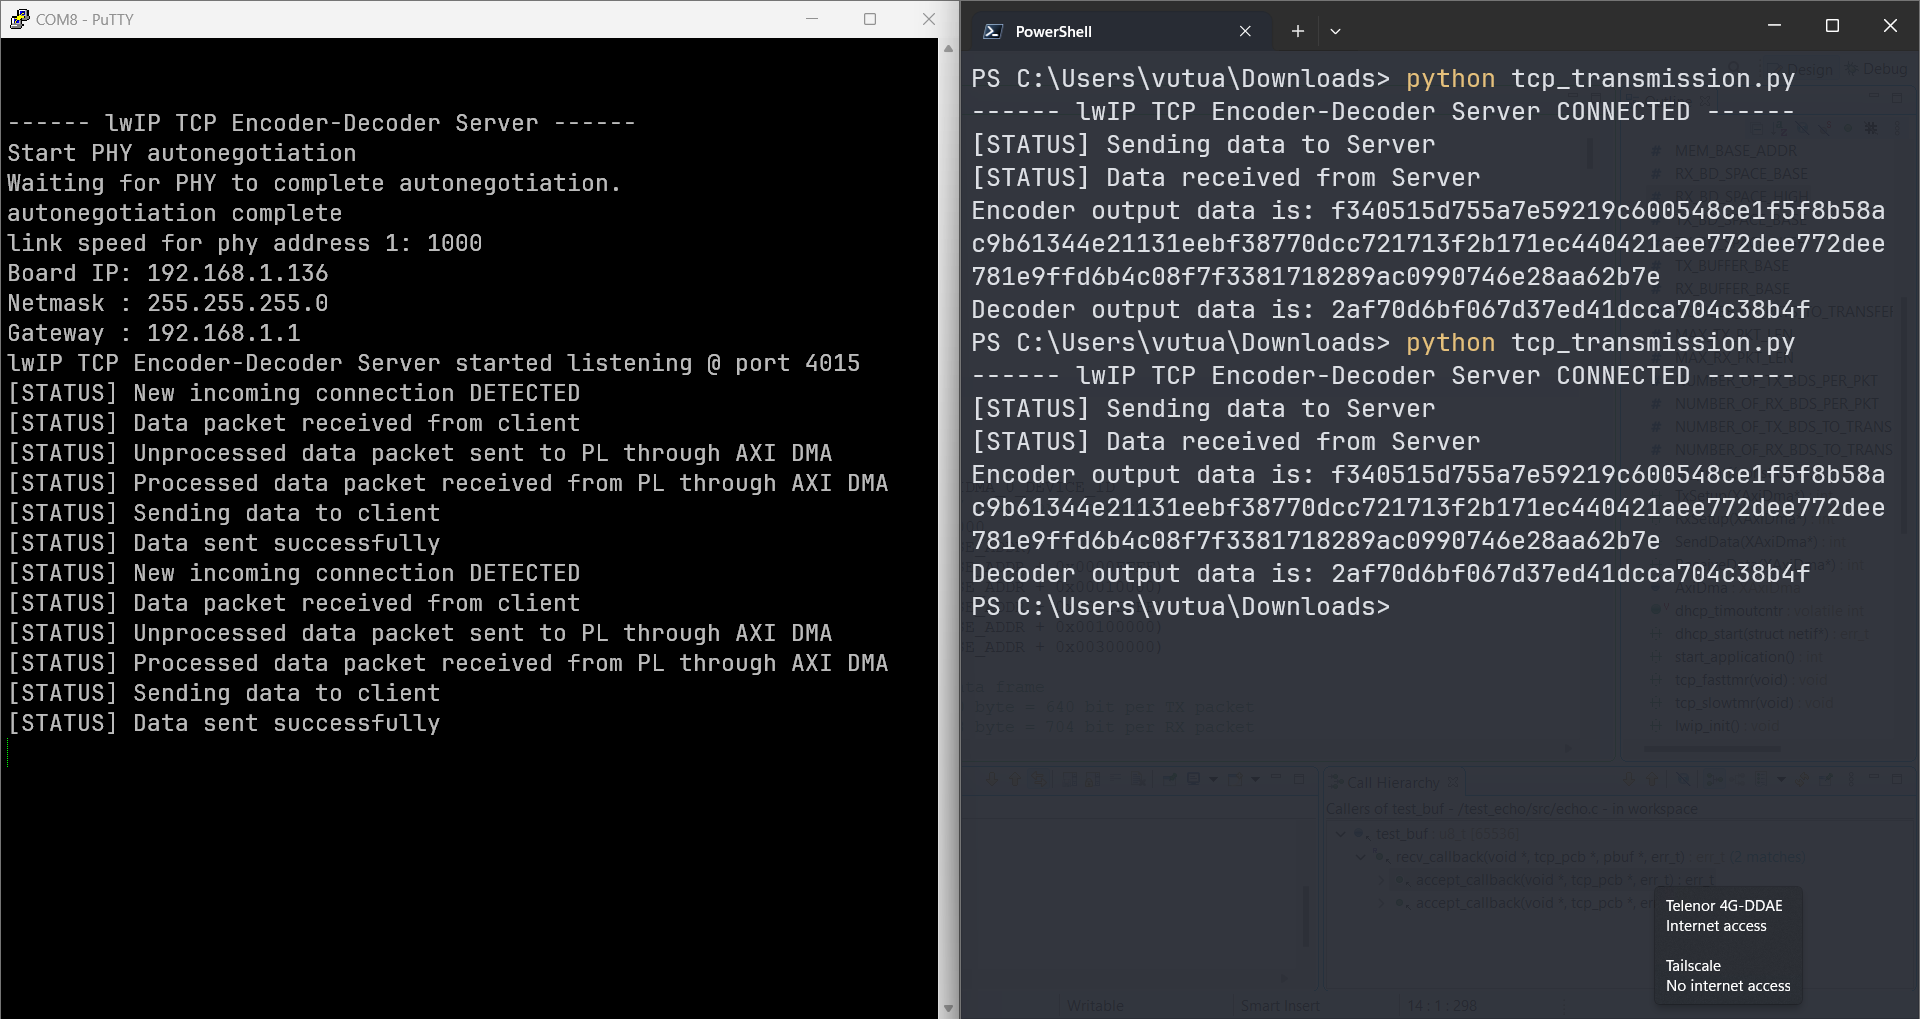
\includegraphics[width=\textwidth, height=0.4\textheight, keepaspectratio]{Hinhve/Chuong 4/tailscale.png}
    \caption{Kiểm thử client kết nối với Tailscale}
    \label{fig:Kiểm thử client kết nối với Tailscale}
\end{figure}

\subsection{Kiểm thử toàn diện hệ thống}
\label{subsection:Kiểm thử toàn diện hệ thống}

Sau khi hoàn thành việc kiểm thử các chức năng cơ bản, quá trình kiểm thử toàn diện toàn hệ thống sẽ được triển khai. Trong giai đoạn này, các bộ dữ liệu mẫu sẽ được tự động sinh ngẫu nhiên bằng phần mềm MATLAB, với các tham số đầu vào tuân thủ theo khoảng giá trị được quy định chi tiết trong Bảng \ref{table: Khoảng giá trị của các tham số}.

\begin{table}[H]
\centering{}
    \caption{Khoảng giá trị của các tham số}
    \begin{tabular}{|p{0.46\linewidth}|p{0.24\linewidth}|}
        \hline
        \textbf{Tham số} & \textbf{Khoảng giá trị} \\ \hline\hline
        Chiều dài ràng buộc  & 4 : 9          \\ \hline
        Tốc độ mã  & 1/2 : 1/3          \\ \hline
        Đa thức sinh cho từng đầu ra   & 0 : $2^{9} - 1$          \\ \hline
        Trạng thái trước của thanh ghi dịch   & 0 : $2^{8} - 1$          \\ \hline
        Dữ liệu cần mã hóa  & 0 : $2^{192} - 1$ \\ \hline
        Dữ liệu cần giải mã & 0 : $2^{384} - 1$ \\ \hline
        \end{tabular}
        \label{table: Khoảng giá trị của các tham số}
\end{table}

MATLAB sẽ được sử dụng để sinh ra tổng cộng 15000 khung dữ liệu ngẫu nhiên, với các tham số đầu vào được giới hạn trong khoảng giá trị đã xác định trước. Toàn bộ tập dữ liệu này sau đó sẽ được chuyển đến Endec Server thông qua giao thức truyền thông đã được thiết lập để tiến hành quá trình kiểm thử chức năng. Dưới đây là các kết quả chi tiết thu được từ quá trình kiểm thử này

\begin{figure}[H]
    \centering
    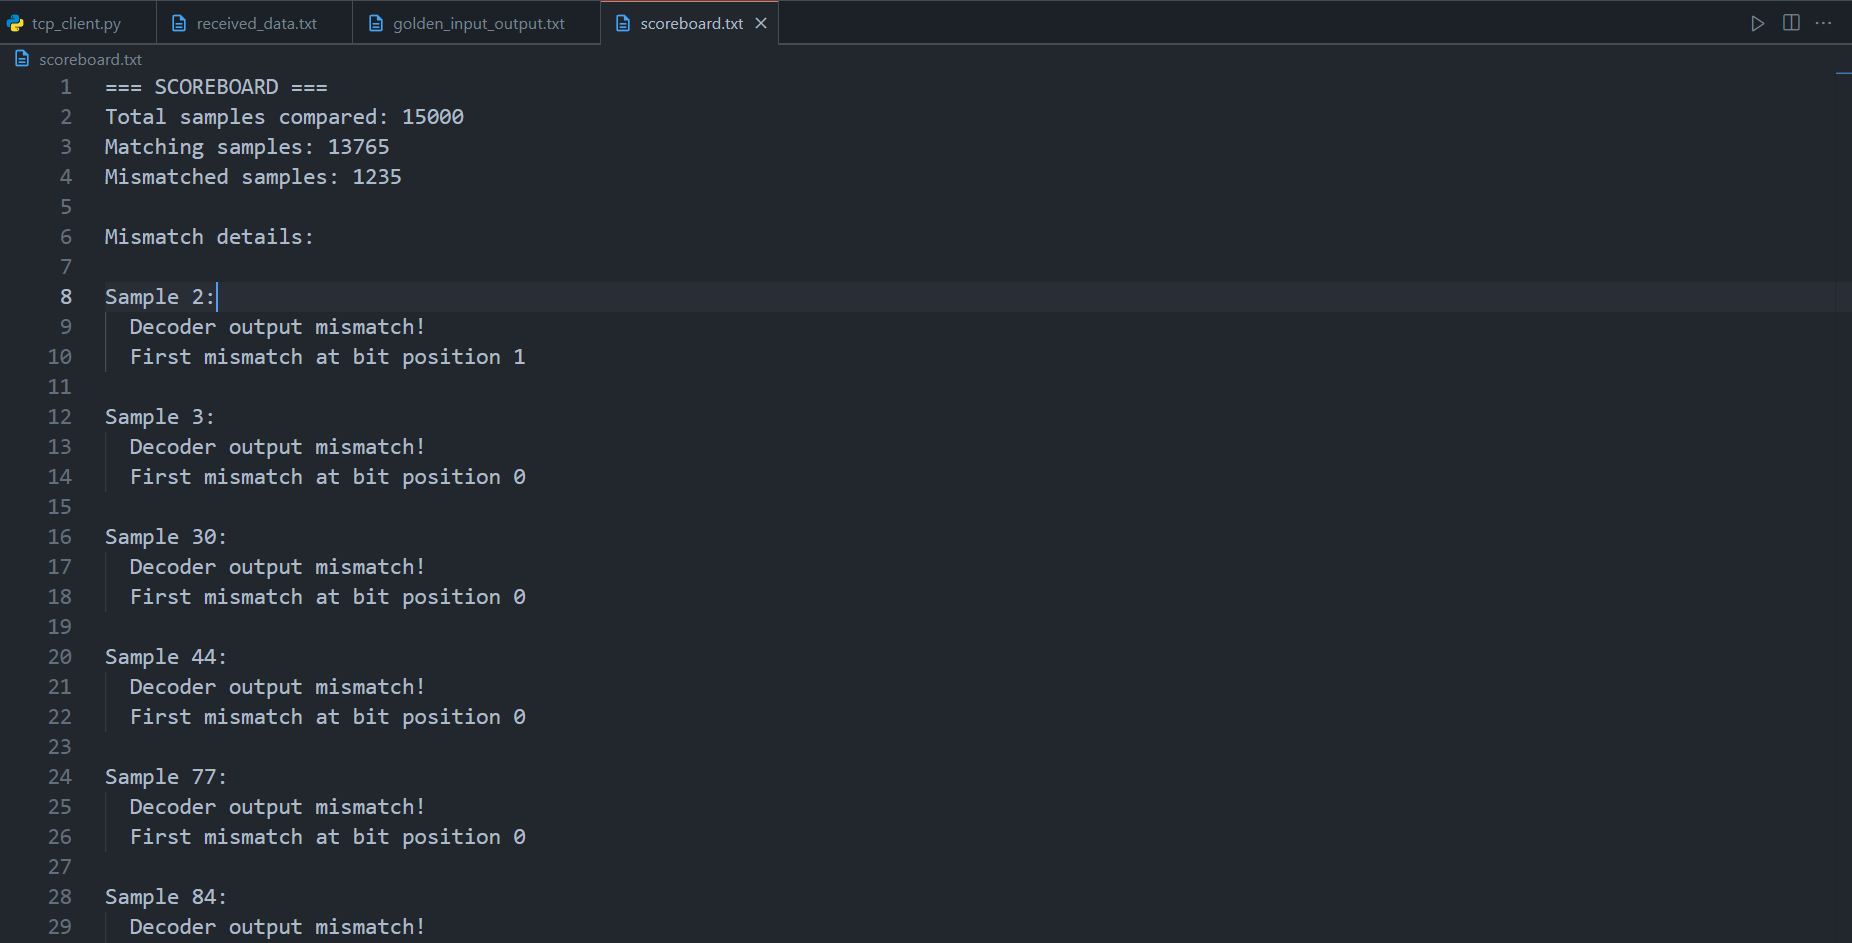
\includegraphics[width=\textwidth, height=0.4\textheight, keepaspectratio]{Hinhve/Chuong 4/data_mismatch.png}
    \caption{Kết quả kiểm thử ban đầu}
    \label{fig:Kết quả kiểm thử ban đầu}
\end{figure}

Hình \ref{fig:Kết quả kiểm thử ban đầu} cho thấy một hiện tượng đáng chú ý: dù dữ liệu mã hóa luôn chính xác, quá trình giải mã lại cho kết quả sai. Tỷ lệ lỗi 8.23\% quan sát được trong hệ thống mã hóa/giải mã có thể bắt nguồn từ việc sử dụng các đa thức sinh không tối ưu. Khi áp dụng phương pháp ngẫu nhiên hóa toàn bộ đa thức sinh, hệ thống có thể tạo ra những đa thức không đạt chuẩn về khoảng cách tự do, thậm chí bao gồm cả các đa thức có khả năng gây lỗi thảm họa (catastrophic) \cite{forney_convolutional_1970}\cite{masseyy_inverses_1968}. Để khắc phục vấn đề này, thuật toán sinh ngẫu nhiên trong MATLAB sẽ được điều chỉnh, chỉ sử dụng các đa thức sinh đã được kiểm chứng và phổ biến trong các hệ thống thông tin thực tế:

\begin{table}[H]
\centering{}
    \caption{Đa thức sinh sau điều chỉnh}
    \begin{tabular}{|p{0.3\linewidth} | p{0.24\linewidth} |p{0.24\linewidth}|}
        \hline
        \textbf{Chiều dài ràng buộc} & \textbf{Tốc độ mã 1/2} & \textbf{Tốc độ mã 1/3}\\ \hline\hline
        4  & 15 $-$ 17 & 15 $-$ 17 $-$ 13          \\ \hline
        5   & 23 $-$ 35 & 25 $-$ 33 $-$ 37         \\ \hline
        6   & 53 $-$ 75 & 55 $-$ 64 $-$ 71          \\ \hline
        7  & 133 $-$ 171 & 133 $-$ 145 $-$ 171 \\ \hline
        8 & 247 $-$ 371 & 247 $-$ 371 $-$ 357 \\ \hline
        9 & 561 $-$ 753 & 557 $-$ 663 $-$ 711 \\ \hline
        \end{tabular}
\end{table}

\begin{figure}[H]
    \centering
    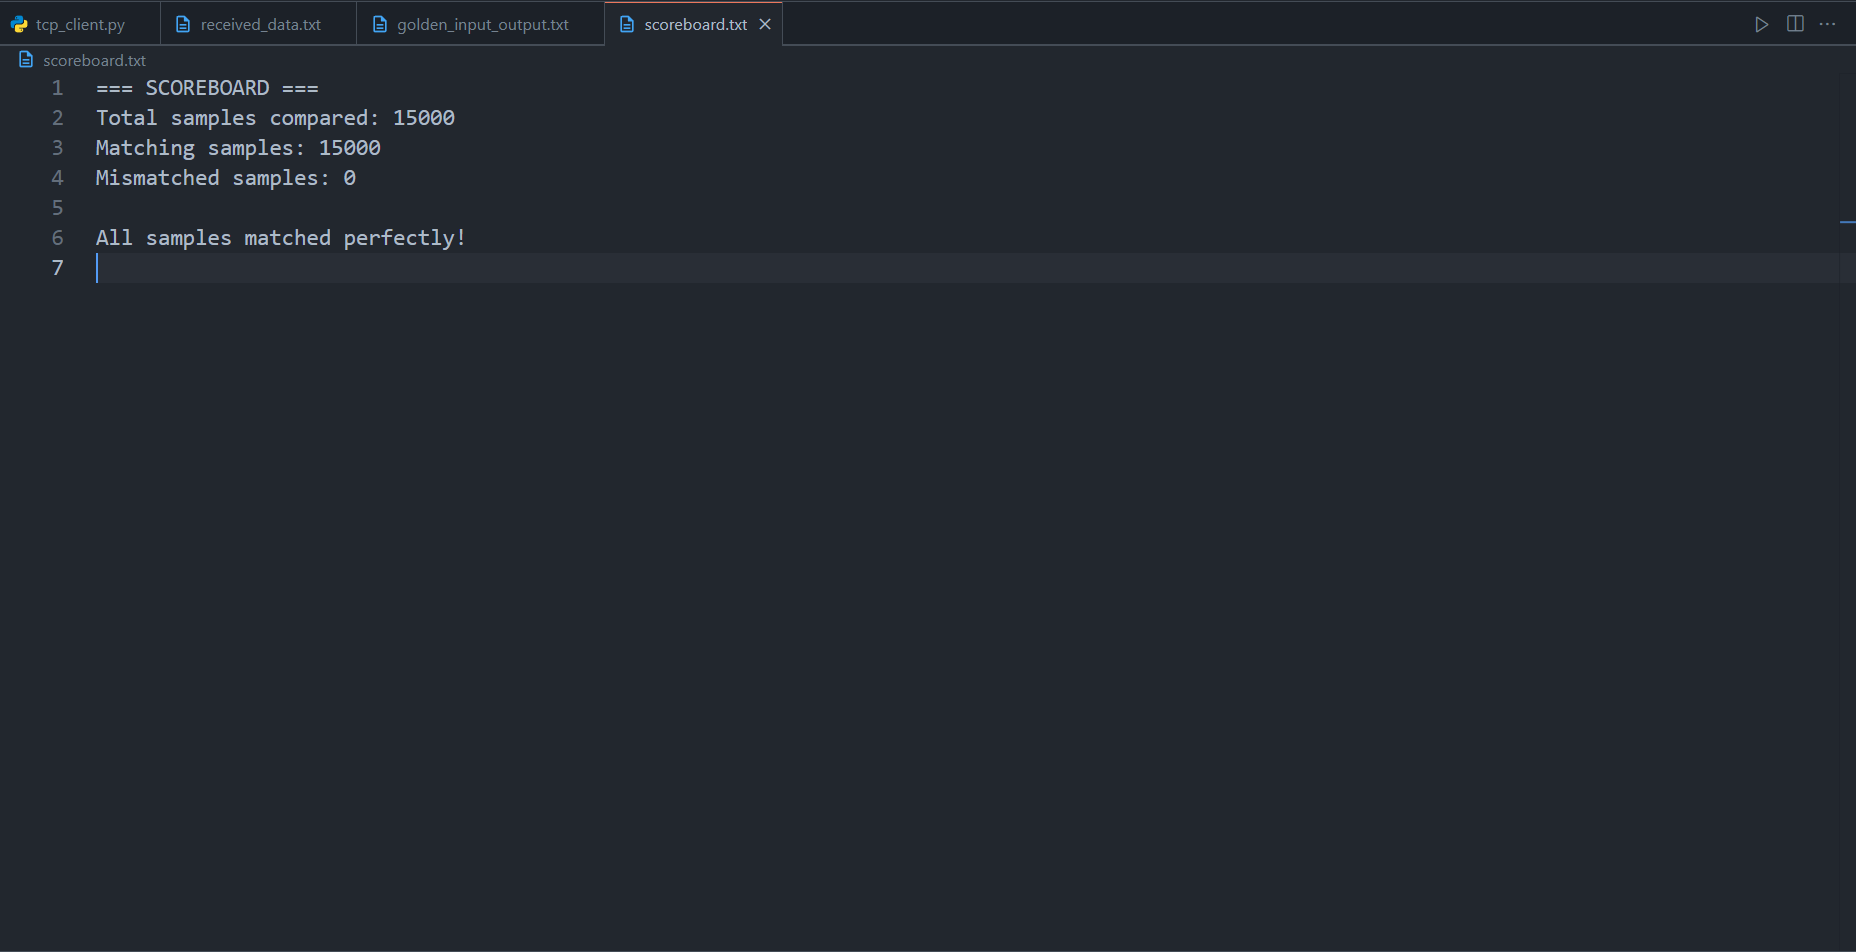
\includegraphics[width=\textwidth, height=0.4\textheight, keepaspectratio]{Hinhve/Chuong 4/data_correct.png}
    \caption{Kết quả kiểm thử sau khi điều chỉnh đa thức sinh}
    \label{fig:Kết quả kiểm thử sau}
\end{figure}

Hình \ref{fig:Kết quả kiểm thử sau} trình bày kết quả kiểm thử hệ thống sau khi đã tối ưu hóa bộ đa thức sinh. Kết quả đạt được độ chính xác 100\% đã khẳng định rằng nguyên nhân gây sai số trong các thử nghiệm trước đó xuất phát từ đặc tính của bộ đa thức sinh mà không phải do lỗi của hệ thống mã hóa/giải mã. Trên cơ sở này, nghiên cứu tiếp tục tiến hành đánh giá thông lượng thực tế của toàn hệ thống.

\begin{figure}[H]
    \centering
    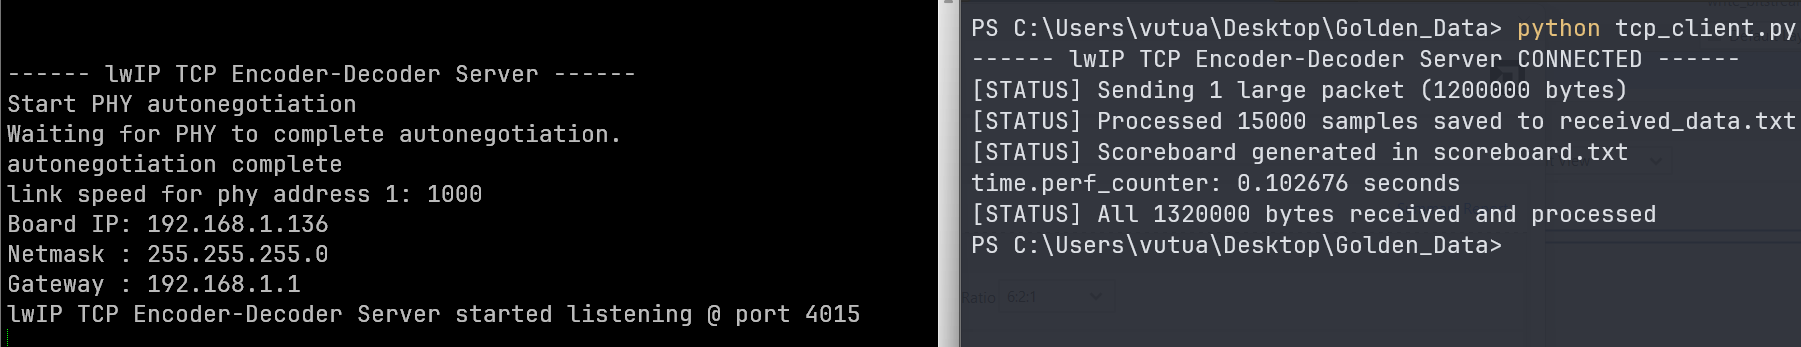
\includegraphics[width=\textwidth, height=0.4\textheight, keepaspectratio]{Hinhve/Chuong 4/throughput.png}
    \caption{Kết quả kiểm thử thông lượng}
    \label{fig:Kết quả kiểm thử thông lượng}
\end{figure}

Theo kết quả trong Hình \ref{fig:Kết quả kiểm thử thông lượng}, hệ thống ghi nhận độ trễ xử lý trung bình là 0.1 giây cho mỗi chu kỳ từ khi client gửi dữ liệu đến khi nhận được dữ liệu đã xử lý. Trên cơ sở 15000 khung dữ liệu thử nghiệm, với thông số kỹ thuật mỗi khung bao gồm 192 bit dữ liệu đầu vào cần mã hóa và 128 bit dữ liệu đầu ra đã được giải mã, ta có thể tính toán được thông lượng của Endec Server thông qua công thức sau: 

\begin{equation}
\text{Thông lượng mã hóa} = \frac{\text{Số bit mã hóa đầu vào}}{\text{Thời gian xử lý}}
\label{eq:enc_throughput}
\end{equation}


\begin{equation}
\text{Thông lượng giải mã} = \frac{\text{Số bit giải mã đầu ra}}{\text{Thời gian xử lý}}
\label{eq:dec_throughput}
\end{equation}

Công thức tính thông lượng (\ref{eq:enc_throughput}) và (\ref{eq:dec_throughput}) dựa vào lượng thông tin hữu dụng mà bên phát/bên thu cần truyền/ nhận. Áp dụng công thức trên, ta có thể tính được thông lượng mã hóa/giải mã của Endec Server lần lượt là 28.8Mbps và 19.2Mbps

\section{Tổng kết}

\subsection{Đánh giá thông số hoạt động của Endec Server}

Trong quá trình phát triển, hệ thống đã trải qua nhiều lần điều chỉnh và tối ưu hóa nhằm cải thiện thông lượng, hiệu suất, khắc phục lỗi và tối ưu tài nguyên. Do đó, việc đánh giá khả năng hoạt động của hệ thống không thể thực hiện trong giai đoạn triển khai giữa chừng mà chỉ có thể tiến hành sau khi đã hoàn thành kiểm thử chức năng và tối ưu hóa hiệu năng. Dưới đây là bảng tổng hợp các thông số của hệ thống sau khi đã vượt qua kiểm thử chức năng và được tối ưu hóa hiệu suất: 

\begin{table}[H]
\centering{}
    \caption{Tài nguyên PL sử dụng}
    \begin{tabular}{|p{0.15\linewidth}|p{0.36\linewidth}|p{0.36\linewidth}|}
        \hline
        \textbf{Tài nguyên} & \textbf{Giá trị sử dụng tuyệt đối} & \textbf{Giá trị sử dụng tương đối} \\ \hline\hline
        LUT  & 43095 & 81\% \\ \hline
        LUTRAM  & 734 & 4\% \\ \hline
        FF  & 33739 & 32\% \\ \hline
        BRAM  & 125 & 89\% \\ \hline
        BUFG  & 2 & 6\% \\ \hline
        \end{tabular}
        \label{table:Tài nguyên PL sử dụng}
\end{table}

Kết quả tổng hợp trong Bảng \ref{table:Tài nguyên PL sử dụng} cho thấy thiết kế hiện đã tối ưu hóa việc sử dụng tài nguyên PL để đạt hiệu năng xử lý cao. Đáng chú ý, tài nguyên LUT đạt mức sử dụng 81\% (43,095 LUT) do yêu cầu xử lý phức tạp của khối add\_compare\_select - nơi cần thực hiện mạng lưới tính toán đồng thời 1024 dịch chuyển cho mỗi bước thời gian. Tuy nhiên, việc vượt ngưỡng 80\% này tiềm ẩn nguy cơ nghẽn tín hiệu khi triển khai phần cứng, vấn đề sẽ được phân tích sâu tại mục \ref{subsection:signal_congestion} trong Chương \ref{chapter:conclusion}.

Mặt khác, tài nguyên FF chỉ đạt 32\% (33,739 FF) do chủ yếu đóng vai trò trung chuyển tín hiệu và không ảnh hưởng đáng kể đến hiệu năng hệ thống. Các tài nguyên khác thể hiện mức sử dụng đa dạng: BRAM đạt 89\% (125 khối) cho thấy việc tận dụng tối đa bộ nhớ, trong khi LUTRAM (4\%) và BUFG (6\%) được sử dụng ở mức khiêm tốn. 

\begin{table}[H]
\centering{}
    \caption{Thông số hoạt động của hệ thống}
    \begin{tabular}{|p{0.6\linewidth}|p{0.15\linewidth}|}
        \hline
        \textbf{Thông số} & \textbf{Giá trị}\\ \hline\hline
        Chiều dài ràng buộc hỗ trợ  & 4 : 9           \\ \hline
        Tốc độ mã hỗ trợ  & 1/2 : 1/3 \\ \hline
        Đa thức sinh hỗ trợ   &  0 : $2^{9} -1$ \\ \hline
        Độ sâu truy ngược  & 64 \\ \hline
        Số bit mã hóa đầu vào trong một khung dữ liệu & 192 bit \\ \hline
        Số bit giải mã đầu ra trong một khung dữ liệu & 128 bit \\ \hline
        Xung nhịp hoạt động & 81.25 MHz \\ \hline
        Công suất tiêu thụ & 1.64 W \\ \hline
        Nhiệt độ khi hoạt động & 43.9\textdegree{}C \\ \hline
        \end{tabular}
        \label{table:Thông số hoạt động của hệ thống}
\end{table}

Như kết quả trình bày trong Bảng \ref{table:Thông số hoạt động của hệ thống}, hệ thống hiện không hỗ trợ chiều dài ràng buộc 3 - một thông số khá phổ biến trong các hệ thống tương tự. Nguyên nhân cụ thể và giải pháp khắc phục cho vấn đề này sẽ được phân tích chi tiết tại mục \ref{subsection:constraint_len3_radix_4} trong Chương \ref{chapter:conclusion}.

Về hiệu năng hoạt động, hệ thống đạt được xung nhịp 81.25 MHz - con số tuy khiêm tốn nhưng cần được đánh giá trong bối cảnh kiến trúc Radix-4 đặc thù của bộ giải mã Viterbi. Nguyên nhân chính giới hạn tốc độ xử lý nằm ở đường truyền tới hạn (Critical Path) trong khối add\_compare\_select, nơi phải thực hiện phép so sánh đồng thời 1024 dịch chuyển trạng thái. Tuy nhiên, cần lưu ý rằng với cơ chế xử lý 2 bit/chu kỳ của kiến trúc Radix-4, hiệu năng thực tế của hệ thống hiện tại ở 81.25 MHz sẽ tương đương với hệ thống với kiến trúc Radix-2 truyền thống hoạt động ở 162.5 MHz khi các điều kiện khác là tương đồng.

Kết quả kiểm thử hệ thống tại mục \ref{subsection:Triển khai phần mềm nhúng và kiểm thử trực tiếp} cho thấy quá trình xử lý mỗi khung dữ liệu cần 209 chu kỳ xung nhịp. Dựa trên thông số xung nhịp hoạt động được trình bày trong Bảng \ref{table:Thông số hoạt động của hệ thống} kết hợp với việc biến đổi các công thức (\ref{eq:enc_throughput}) và (\ref{eq:dec_throughput}), ta có thể xác định thông lượng hệ thống khi giao tiếp với AXI DMA thông qua các công thức tính toán sau:

\begin{equation}
\text{Thông lượng mã hóa} = \frac{\text{Số bit mã hóa đầu vào trong một khung dữ liệu}}{\text{Chu kỳ xử lý}\times\frac{1}{\text{Xung nhịp hoạt động}} }
\label{eq:enc_frame_throughput}
\end{equation}

\begin{equation}
\text{Thông lượng giải mã} = \frac{\text{Số bit giải mã đầu ra trong một khung dữ liệu}}{\text{Chu kỳ xử lý}\times\frac{1}{\text{Xung nhịp hoạt động}} }
\label{eq:dec_frame_throughput}
\end{equation}

Với kiến trúc xử lý song song độc lập giữa các tác vụ TX và RX đã được mô tả trong mục \ref{subsection:Thiết kế khối endec_interface}, hệ thống đạt được độ ổn định cao khi xử lý mỗi khung dữ liệu trong 209 chu kỳ xung nhịp. Điều này khẳng định tính chính xác của các công thức (\ref{eq:enc_frame_throughput}) và (\ref{eq:dec_frame_throughput}) trong việc đánh giá thông lượng hệ thống khi tích hợp với AXI DMA. Dựa trên kết quả kiểm thử thực tế thu được tại mục \ref{subsection:Kiểm thử toàn diện hệ thống}, thông lượng hệ thống qua các giai đoạn kiểm thử được tổng hợp thành bảng sau:

\begin{table}[H]
\centering{}
    \caption{Thông lượng xử lý qua các giai đoạn của hệ thống}
    \begin{tabular}{|p{0.28\linewidth}|p{0.3\linewidth}|p{0.3\linewidth}|}
        \hline
        \textbf{Giai đoạn} & \textbf{Thông lượng mã hóa} & \textbf{Thông lượng giải mã}\\ \hline\hline
        Qua AXI DMA  & 74.6 Mbps & 49.8 Mbps \\ \hline
        Qua lwIP TCP Server  & 28.8 Mbps & 19.2 Mbps \\ \hline
        \end{tabular}
        \label{table:Thông lượng xử lý qua các giai đoạn của hệ thống}
\end{table}

Kết quả so sánh từ Bảng \ref{table:Thông lượng xử lý qua các giai đoạn của hệ thống} cho thấy thông lượng hệ thống giảm xuống chỉ còn 39\% khi xử lý qua lwIP TCP Server so với khi sử dụng trực tiếp AXI DMA. Sự sụt giảm đáng kể này bắt nguồn từ ba yếu tố chính. Thứ nhất, chi phí điều khiển (overhead) cho mỗi tác vụ xử lý đã làm giảm hiệu suất tổng thể. Thứ hai, hệ thống hiện mới chỉ khai thác một nhân xử lý trong khi board PYNQ-Z2 được trang bị bộ xử lý lõi kép, dẫn đến việc chưa tận dụng hết tiềm năng phần cứng. Thứ ba, việc AXI DMA Controller hoạt động ở chế độ polling thay vì interrupt khiến PS phải chờ DMA hoàn thành tác vụ trước khi chuyển sang xử lý lwIP TCP Server, tạo ra các khoảng thời gian chết không cần thiết. Những hạn chế này kết hợp lại đã ảnh hưởng đáng kể đến thông lượng xử lý của toàn hệ thống.
 

\subsection{So sánh với các hệ thống khác}

Hệ thống Endec Server được phát triển với mục tiêu hướng đến người dùng không chuyên, do đó cần có sự so sánh khả năng hoạt động với các giải pháp tương tự trên thị trường. Hiện nay, các bộ mã hóa tích chập và giải mã Viterbi thường được triển khai dưới dạng module tích hợp trong vi mạch, thiết kế FPGA hoặc chương trình chạy trên CPU/GPU. Tuy nhiên, các giải pháp này đều có những hạn chế chung như không phổ biến, không hỗ trợ đầy đủ các cấu hình thông dụng, không có thông số chuẩn hóa và đặc biệt là khó tiếp cận đối với người dùng phổ thông, khiến chúng trở thành tiêu chí tham chiếu không lý tưởng để đánh giá hệ thống hiện tại.

Trong bối cảnh đó, MATLAB nổi lên như một lựa chọn tham chiếu phù hợp mặc dù có những nhược điểm về hiệu năng và tối ưu tài nguyên. Ưu điểm nổi bật của MATLAB là tính phổ biến cao và dễ tiếp cận đối với đa số người dùng không chuyên. Mặc dù thông lượng xử lý phụ thuộc nhiều vào cấu hình phần cứng nền tảng, nhưng với cùng một thuật toán, kết quả từ MATLAB vẫn có thể cung cấp một chuẩn đánh giá tương đối khách quan. Chính những yếu tố này khiến MATLAB trở thành điểm tham chiếu hợp lý để đánh giá hiệu năng của hệ thống Endec Server trong nghiên cứu hiện tại. Sau đây là bảng so sánh giữa MATLAB và Endec Server dưới góc nhìn của người dùng với các tiêu chí khác nhau: 

\begin{table}[H]
\centering

\begin{threeparttable}

\caption{So sánh MATLAB và Endec Server}
\begin{tabular}{|p{0.26\linewidth}|p{0.31\linewidth}|p{0.31\linewidth}|}
    \hline
    \textbf{Tiêu chí} & \textbf{MATLAB} & \textbf{Endec Server} \\ \hline\hline
    Quá trình cài đặt & Cần có license và tải về MATLAB & Kết nối với Mesh Network qua Tailscale \\ \hline 
    Tài nguyên yêu cầu & Lớn, không phù hợp với các hệ thống nhúng & Có kết nối mạng \\ \hline
    Tài nguyên sử dụng & Tiêu tốn tài nguyên khi thực hiện mã hóa/giải mã & Gần như không tiêu tốn tài nguyên \\ \hline
    Công suất tiêu thụ & 45 W (CPU)\tnote{*} & 1.64 W \\ \hline
    Độ ổn định & Dễ gặp hiện tượng treo, nghẽn dữ liệu & Luôn hoạt động ổn định \\ \hline
    \multirow{2}{*}{Thông lượng xử lý} 
      & Mã hóa: 1.31 Mbps\tnote{*} & Mã hóa: 28.8 Mbps \\ 
      & Giải mã: 0.23 Mbps\tnote{*} & Giải mã: 19.2 Mbps \\ \hline 
\end{tabular}
\begin{tablenotes}
\item[*] Được thực hiện trên CPU Ryzen 5 5600H
\end{tablenotes}

\end{threeparttable}

\label{table:So sánh MATLAB và Endec Server}
\end{table}

Qua bảng so sánh giữa MATLAB và Endec Server, có thể thấy rõ sự khác biệt đáng kể về hiệu suất và hiệu quả năng lượng giữa hai giải pháp. MATLAB đòi hỏi phải có bản quyền và cài đặt phần mềm cồng kềnh, trong khi Endec Server chỉ cần kết nối mạng đơn giản qua Tailscale. Về mặt tài nguyên, MATLAB tiêu tốn nhiều năng lượng với mức tiêu thụ trung bình là 45W cho các CPU tầm trung phổ biến, ngược lại Endec Server hoạt động ổn định với mức tiêu thụ năng lượng cực thấp chỉ 1.64W.

Khả năng hoạt động ổn định của Endec Server đến từ việc kết hợp hài hòa giữa kiến trúc phần cứng xác định và phần mềm được tối ưu hóa cao. Trên khối xử lý lập trình được PL, hệ thống đạt được tính xác định thời gian thực nhờ kiến trúc xử lý song song cứng, cho phép thực hiện các tác vụ xử lý tín hiệu số một cách độc lập và ổn định mà không phụ thuộc vào hệ điều hành. Điều này giải thích tại sao Endec Server có thể duy trì hoạt động liên tục trong khi MATLAB dễ gặp phải tình trạng treo hệ thống hay nghẽn dữ liệu. Ở khối xử lý ứng dụng PS, giải pháp sử dụng phương pháp lập trình baremetal giúp hệ thống đạt được sự ổn định tối đa. Bằng cách loại bỏ hoàn toàn hệ điều hành, hệ thống tránh được các vấn đề về tranh chấp tài nguyên và giảm thiểu độ trễ xử lý.

Ưu điểm về tính ổn định này càng được khẳng định thông qua hiệu suất xử lý vượt trội của Endec Server. Trong khi MATLAB chỉ đạt được thông lượng mã hóa 1.31 Mbps và giải mã 0.23 Mbps, thì Endec Server có thể xử lý lên tới 28.8 Mbps cho mã hóa và 19.2 Mbps cho giải mã. Sự khác biệt này đến từ việc tối ưu hóa toàn diện từ phần cứng đến phần mềm, đặc biệt là khả năng xử lý tín hiệu số hiệu quả với nhiễu được kiểm soát chặt chẽ. Mặc dù có sự suy giảm đáng kể về thông lượng do quá trình truyền tải TCP qua lwIP TCP Server, Endec Server vẫn duy trì được hiệu suất ấn tượng.

Kết quả so sánh đã chứng minh rằng Endec Server không chỉ đáp ứng được các yêu cầu kỹ thuật đặt ra ban đầu mà còn thể hiện rõ những ưu điểm vượt trội về hiệu suất và tiết kiệm năng lượng so với phương pháp truyền thống sử dụng MATLAB. Điều này khẳng định tính khả thi và giá trị ứng dụng thực tiễn của giải pháp Endec Server trong các hệ thống thực tế.

\end{document}
